\documentclass[11pt,a4paper]{article}
\usepackage[margin=1in]{geometry}
\usepackage[utf8]{inputenc}
\usepackage{authblk}
\usepackage[english]{babel}
\usepackage{amsmath}
\usepackage{amsfonts}
\usepackage{amssymb}
\usepackage{amsthm}
\usepackage{bbm}
\usepackage{mathabx} % for \ldbrack, \rdbrack
\usepackage{graphicx}
\usepackage{natbib}
\bibliographystyle{abbrvnat}
\usepackage{nicefrac}
\usepackage{todonotes}
\usepackage{lineno}
\linenumbers
\usepackage{comment}
\usepackage[acronym]{glossaries}
\usepackage{xcolor}
\usepackage{url}
\usepackage{hyperref}
\hypersetup{
    colorlinks=true,
    linkcolor=blue,
    filecolor=magenta,
    urlcolor=blue,
    citecolor=black
}
\usepackage[most]{tcolorbox}
\usepackage{nicefrac}

%%% MATHS COMMANDS %%%
\newtheorem{lemma}{Lemma}
\newtheorem{definition}{Definition}
\newcommand{\Cov}{\mathbb{C}\text{ov}}
\newcommand{\Cor}{\mathbb{C}\text{or}}
\newcommand{\Var}{\mathbb{V}\text{ar}}
\newcommand{\Prob}{\text{Pr}}
\newcommand{\N}{\mathcal{N}}
\renewcommand{\P}{\mathbb{P}}
\newcommand{\E}{\mathbb{E}}
\newcommand{\ident}[2]{\ldbrack#1=#2\rdbrack}

\newcommand{\bsymb}[1]{\boldsymbol{#1}}

\newcommand{\ppath}{\mathcal{P}}
\newcommand{\sibs}{\mathcal{S}}
\newcommand{\nodes}{\mathcal{N}}
\newcommand{\leT}{\le_T}
\newcommand{\geT}{\ge_T}
\newcommand{\nleT}{\nleq_T}
\newcommand{\pluseq}{\mathrel{+}=}
\newcommand{\minuseq}{\mathrel{-}=}
\newcommand{\timeseq}{\mathrel{*}=}
\newcommand{\diveq}{\mathrel{/}=}

\setlength{\marginparwidth}{2cm}

%%% COMMENTS %%%
\newcommand{\brieuc}[1]{{\textcolor{purple}{{\bf Brieuc:} #1}}}
\newcommand{\peter}[1]{{\textcolor{orange}{{\bf Peter:} #1}}}
\newcommand{\jerome}[1]{{\textcolor{green}{{\bf Jerome:} #1}}}
\newcommand{\gregor}[1]{{\textcolor{blue}{{\bf Gregor:} #1}}}
\newcommand{\georgia}[1]{{\textcolor{blue}{{\bf Georgia:} #1}}}
\newcommand{\luke}[1]{{\textcolor{cyan}{{\bf Luke:} #1}}}

%%% ACRONYMS and things %%%
\newcommand{\eGRM}{\texttt{eGRM}}
\newcommand{\tskit}{\texttt{tskit}}
\newcommand{\scipy}{\texttt{scipy}}
\newcommand{\eigh}{\texttt{eigh}}
\newcommand{\eigsh}{\texttt{eigsh}}
\newcommand{\scikitallel}{\texttt{scikit-allel}}
\newcommand{\ARGneedlelib}{\texttt{ARG-needle-lib}}
\newcommand{\tsGRM}{\texttt{ts.genetic\_relatedness\_matrix}}
\newcommand{\tsGR}{\texttt{ts.genetic\_relatedness}}
\newcommand{\tsGRw}{\texttt{ts.genetic\_relatedness\_weighted}}
\newcommand{\tsPCA}{\texttt{ts.pca}}
\newcommand{\msprime}{\texttt{msprime}}

\newacronym{grm}{GRM}{genetic relatedness matrix}
\newacronym{arg}{ARG}{ancestral recombination graph}

% These macros are borrowed from TAOCPMAC.tex
\newcommand{\slug}{\hbox{\kern1.5pt\vrule width2.5pt height6pt depth1.5pt\kern1.5pt}}
\def\xskip{\hskip 7pt plus 3pt minus 4pt}
\newdimen\algindent
\newif\ifitempar \itempartrue % normally true unless briefly set false
\def\algindentset#1{\setbox0\hbox{{\bf #1.\kern.25em}}\algindent=\wd0\relax}
\def\algbegin #1 #2{\algindentset{#21}\alg #1 #2} % when steps all have 1 digit
\def\aalgbegin #1 #2{\algindentset{#211}\alg #1 #2} % when 10 or more steps
\def\alg#1(#2). {\medbreak % Usage: \algbegin Algorithm A (algname). This...
  \noindent{\bf#1}({\it#2\/}).\xskip\ignorespaces}
\def\kalgstep#1.{\ifitempar\smallskip\noindent\else\itempartrue
   \hskip-\parindent\fi
   \hbox to\algindent{\bf\hfil #1.\kern.25em}%
   \hangindent=\algindent\hangafter=1\ignorespaces}

\newcommand{\algstep}[3]{\kalgstep #1 [#2] #3 }
\newenvironment{taocpalg}[3]{%
\vspace{1em}%
\algbegin Algorithm #1. ({#2}). #3 }
{\vspace{1em}}

\newcommand{\algorithmref}[1]{#1}

% This doesn't seem to be working, unusually?
% from http://tex.stackexchange.com/questions/43648/why-doesnt-lineno-number-a-paragraph-when-it-is-followed-by-an-align-equation/55297#55297
\ifcsname{patchAmsMathEnvironmentForLineno}\endcsname
    \newcommand*\patchAmsMathEnvironmentForLineno[1]{%
      \expandafter\let\csname old#1\expandafter\endcsname\csname #1\endcsname
      \expandafter\let\csname oldend#1\expandafter\endcsname\csname end#1\endcsname
      \renewenvironment{#1}%
         {\linenomath\csname old#1\endcsname}%
         {\csname oldend#1\endcsname\endlinenomath}}%
    \newcommand*\patchBothAmsMathEnvironmentsForLineno[1]{%
      \patchAmsMathEnvironmentForLineno{#1}%
      \patchAmsMathEnvironmentForLineno{#1*}}%
    \AtBeginDocument{%
    \patchBothAmsMathEnvironmentsForLineno{equation}%
    \patchBothAmsMathEnvironmentsForLineno{align}%
    \patchBothAmsMathEnvironmentsForLineno{flalign}%
    \patchBothAmsMathEnvironmentsForLineno{alignat}%
    \patchBothAmsMathEnvironmentsForLineno{gather}%
    \patchBothAmsMathEnvironmentsForLineno{multline}%
\fi


\title{On ARGs, pedigrees, and genetic relatedness matrices} % matri-cees

\author[1]{Brieuc Lehmann}
\author[2]{Hanbin Lee}
\author[3]{Luke Anderson-Trocm\'{e}}
\author[4]{Jerome Kelleher}
\author[5]{Gregor Gorjanc}
\author[6,7]{Peter L. Ralph}

\affil[1]{\small{Department of Statistical Science, University College London, WC1E 7HB, UK}}
\affil[2]{\small{Department of Statistics, University of Michigan, Ann Arbor MI 48109, USA}}
\affil[3]{\small{Department of Human Genetics, University of Chicago, Chicago IL 60637, USA}}
\affil[4]{\small{Big Data Institute, Li Ka Shing Centre for Health Information and Discovery, University of Oxford, OX3 7LF, UK}}
\affil[5]{\small{The Roslin Institute and Royal (Dick) School of Veterinary Studies, University of Edinburgh, UK}}
\affil[6]{\small{Institute of Ecology and Evolution, University of Oregon, Eugene OR 97402, USA}}
\affil[7]{\small{Department of Data Science, University of Oregon, Eugene OR 97402, USA}}

\date{\small{\today{}}}

\begin{document}

\maketitle

\section*{Abstract}

Genetic relatedness is a central concept in genetics,
underpinning studies of population and quantitative genetics in human, animal, and plant settings.
%
It is typically stored as a genetic relatedness matrix (GRM),
whose elements are pairwise relatedness values between individuals.
%
This relatedness has been defined in various contexts
based on pedigree, genotype, phylogeny, coalescent times,
and, recently, ancestral recombination graph (ARG).
%
% The ARG-based GRMs were found to better capture the structure of a population and
% improve association studies relative to the genotype GRM.
%
Here, we discuss the different definitions of relatedness in a unifying context,
making use of the additive model of a quantitative trait
to provide a definition of ``branch relatedness'' and the corresponding branch GRM.
%
We explore the relationship between branch relatedness and pedigree relatedness through a case study of French-Canadian individuals that have a known pedigree.
%
Through the tree sequence encoding of an ARG, we then derive an efficient algorithm for computing products between the branch GRM and a general vector, without explicitly forming the branch GRM.
%
This algorithm leverages the sparse encoding of genomes with the tree sequence and hence enables large-scale computations with the branch GRM.
%
We demonstrate the power of this algorithm by developing
a randomized principal components algorithm for tree sequences
that easily scales to millions of genomes.
%
All algorithms are implemented in the open source \tskit{} Python package.
%
Taken together, this work consolidates the different notions of relatedness as branch relatedness
and by leveraging the tree sequence encoding of an ARG it provides efficient algorithms
that enable computations with the branch GRM that scale to mega-scale genomic datasets.


\section{Introduction}


% --- BRIEF INTRO -------------------------------------------------------------

% Paragraph on Background
Relatedness is a fundamental concept in genetics.
%
In its most general sense, genetic relatedness refers to the notion of
similarity between individuals' genomes.
%
These similarities are usually organised as a pairwise comparison of the
genomes within an individual and between individuals, or groups of
individuals.
%
As one of the central genetic concepts, relatedness is used in many
applications \citep{weir2006genetic, speed2015relatedness}.
%
For example, it has been used to describe genetic variation within and between individuals
and groups of individuals in population genetics
\citep{crow2009introduction, charlesworth2010elements},
to analyse phenotype covariation between close and distant relatives in
quantitative genetics \citep{falconer1996introduction, lynch1998genetics},
and to estimate genetic changes in phenotypic variation over time in
evolutionary genetics \citep{walsh2018evolution, arnold2023evolutionary}.
%
For a set of individuals, we store their pairwise relatedness in a genetic relatedness matrix (GRM).
%
Over time, genetic relatedness and GRMs have been defined according to
pedigree \citep{fisher1919correlation, wright1922coefficients},
genotype \citep{cotterman1940calculus, malecot1948mathematiques, malecot1969mathemathics},
phylogeny \citep{felsenstein1985phylogenies,lynch1991methods},
coalescent times \citep{slatkin1991inbreeding}, and
% moving this two paragraphs down -> let's keep it here to create a link to the next paragraph
% (as in why ARG
recently, ancestral recombination graph \citep{tsambos2022efficient, fan2022genealogical, zhang2023biobank}.
%
% \textcolor{red}{We review the standard definitions in Appendix: A Brief History of Genetic Relatedness}.
    
% Paragraph on ARG and relatedness
Ancestral recombination graphs (ARGs) 
describe the network of inheritance relations between a set of individuals
via the action of recombination and mutation within a (usually implicit) pedigree
% JK: rationale for these 4 refs is that they are all review papers from the past
% year. This covers the various different modern perspectives of what an ARG is.
\citep{brandt2024promise, lewanski2024era, wong2023general, nielsen2024inference},
and so provide a common framework in which to consider
the various concepts of relatedness.
%
Although ARGs are not directly observable,
there has been significant recent progress in inferring ARGs from a sample of DNA sequences
\citep{rasmussen2014genome,speidel2019method, kelleher2019inferring, zhang2023biobank, deng2024robust, gunnarsson2024scalable}.
%
This has been accompanied by computational advances that enable
the highly efficient storage and processing of ARGs
\citep{kelleher2016efficient, zhu2024variance, dehaas2024enabling}.
%
In this paper we make use of the \textit{succinct tree sequence} 
ARG encoding
\citep{ralph2020efficiently, wong2023general}
made available through the \tskit{} library.

% Paragraph on Branch relatedness
In addition to providing a unifying framework,
ARGs have led to new formulations of relatedness.
%
The ``eGRM'' of \citet{fan2022genealogical}
defines the relatedness between two individuals
in terms of the total area of branches in the ARG that are ancestral to both,
similar to previous single-tree definitions \citep{slatkin1991inbreeding}.
%
\citet{fan2022genealogical} showed this is the expected genotype relatedness
under a Poisson model of mutation,
a special case of a more general duality between ``branch''
and ``site'' statistics \citep{ralph2019empirical, ralph2020efficiently}.
%
The same concept was used by \citet{zhang2023biobank},
although with different terminology,
who connected their definition of the ``ARG-GRM'' to
the time to most recent common ancestor (TMRCA)
of a single tree \citep{slatkin1991inbreeding, mcvean2009genealogical}.
%
There are many different notions of relatedness (see Box 1 for a 
brief overview), usually defined as an expectation of some 
quantity (e.g., pedigree relatedness is the expected genetic identity within a pedigree).
We therefore use the more precise terms 
``branch relatedness'' and ``branch GRM'' 
rather than previously proposed ``eGRM'' or ``ARG-GRM'' 
to avoid confusion.

% Paragraph on Uses of branch GRM
Recent applications of these methods have highlighted the advantages of
using branch information to improve genetic analyses.
%
\citet{fan2022genealogical} demonstrate that the branch GRM (their ``eGRM'')
better describes population structure relative to the corresponding genotype GRM,
even when based on the same genetic information,
and can provide time-resolved characterisations of population structure
by considering shared branch areas on particular subsets of the ARG
defined by specific time intervals.
%
An application of ``eGRM'' has also improved mapping quantitative trait loci
in the presence of allelic heterogeneity and in understudied populations \citep{link2023tree}.
%
\citet{tsambos2022efficient} developed a method
to find DNA segments that are identical-by-descent (IBD) for pairs of individuals in a given ARG and
then summarise these outputs, possibly as an ``IBD GRM'',
which provides an ARG-based analogue to the pedigree GRM.
%
\citet{zhang2023biobank} use a branch GRM (their ``ARG-GRM'')
to estimate heritability and to perform a ``genealogy-wide association scan'',
showing that this approach is more powerful at detecting the effect of rare variants
than association analysis on SNP array genotypes imputed to whole-genome sequence genotypes.

% --- GAP ---------------------------------------------------------------------

% Paragraph on The gap
The scalability of current ARG-based relatedness methods, however, is constrained by
their need generate and store the full branch GRM. As the GRM encodes all 
pairwise relationships among $n$ samples, it requires at least $O(n^2)$
time and space to compute. 
Several datasets, currently available and of core interest for these 
methods, consist of hundreds of thousands of 
samples~\citep{caulfield2017national,turnbull2018100,
bycroft2018genome,backman2021exome,Ros-Freixedes2022pig_wgs_variants,
halldorsson2022sequences,uk2023whole,all2024genomic}
and genomic datasets with millions of samples will soon be 
available~\citep{stark2024call,cook2025our}.
At this scale, algorithms with quadratic time and space complexity are simply
not feasible, and there is a pressing need for more efficient approaches.
It is important to note, however, that the GRM itself is often not the goal;
rather, we are usually interested in what we can do \emph{with} the GRM.
Applications such as principal component analysis (PCA), for example, are
defined in terms of core linear algebra operations performed on the GRM,
and the outputs are of much smaller dimension. Given that all the information
in a GRM is encoded in an ARG, there is the possibility that we can bypass
generating large intermediate matrices and instead compute the quantities
of interest directly.

% to store the full branch GRM in memory, limiting downstream analyses
% such as principal component analysis (PCA) to datasets of 10,000 to 100,000
% individuals, depending on available computational resources. However, many of
% these analyses can be performed using linear algebra techniques that rely
% solely on matrix-vector operations. That is, these algorithms require only the
% product of the matrix with an arbitrary vector, eliminating the need to store
% the full matrix. 

% Efficient algorithms for computing such matrix-vector products
% can therefore significantly enhance the scalability of downstream analyses.
% \todo[inline]{Add a bit more specificity around how PCA can be performed using
% matrix-vector operations, or examples of other downstream tasks that can be
% done with matrix-vector operations?}

%
%Operationally, \citet{fan2022genealogical} shifted the estimation of relatedness from summing over loci of a genotype matrix and for each locus evaluating genotype similarity between samples (for genotype GRM) to summing over local trees of an ARG and for each local tree evaluating time between samples' MRCA and the root (for branch GRM).
%
%Iterating over local trees can be computationally expensive for large genomic datasets with a huge number of past recombination events, and hence a huge number of local trees.
%
% \peter{I think this is true: Both} \citet{fan2022genealogical} and
% \gregor{Peter: they did it to derive, but not to do computations}
%\citet{zhang2023biobank} also approximate the branch GRM by sampling new mutations on the branches of the ARG and computing the genotype GRM from these mutations, and demonstrate that this approach converges to the true branch GRM with high mutation rates, in line with the branch-site duality \citep{ralph2019empirical, ralph2020efficiently}.
%
%Although these methods have used branch GRM in downstream analyses, such as principal component analysis (PCA), estimation of heritability, and genome-wide associations, each of these approaches requires storing the full branch GRM in memory, limiting analyses between 10,000 and 100,000 individuals (depending on the available computational resources).

% --- AIM ---------------------------------------------------------------------

% Paragraph on The aim
In this paper, we explore the relationships between different notions of relatedness and
describe several algorithms to perform computations of, and with, the branch GRM.
%
Specifically, we show how branch relatedness arises as
the covariance of a trait process evolving along the branches of an ARG,
and how this relates to other measures of relatedness.
%
We undertake a comparison of pedigree and branch relatedness
for simulated data from a real pedigree of the French-Canadian population of
\citet{andersontrocme2023genes},
illustrating the variability of the branch GRM within a fixed pedigree.
%
% We describe a procedure to compute the entire branch GRM by efficiently computing TMRCAs
% using the Schieber-Vishkin algorithm \citep{Schieber1988On}.
%
We also develop a new algorithm to perform efficient branch GRM-vector product,
which avoids storing the full branch GRM in memory.
%
This facilitates the use of the randomised singular value decomposition \citep{halko2011findingstructure}
for PCA of over a million samples.
%
All computations are demonstrated using Python \tskit{} library
\citep{ralph2020efficiently, kelleher2024tskit}.


% NOTE: the text for the "results" ended up in the methods 
% section because that was where most of the actual results
% were, and I'm trying to minimise the size of the diff to 
% avoid confusing Overleaf
\section{Results}

% See notation.tex for notation used throughout the paper!

%% OUTLINE (not comprehencive, notes for bits Peter & Hanbin will edit)
% Tie loose threads together of different views on relatedness,
%   in the context of the tree sequence:
%   make it precise, but easy
%   probably only biallelic markers
%   (this exists, and is about right)
% Algorithms: big-picture; details in the appendix
%   describe alg for simulating traits
%   point out matrix-vector is of a similar form
%   explain how to use matrix-vector toi efficiently do PCA

% --- INTRO TO METHODS ---------------------------------------------------

% Paragraph on The overview of methods
We begin by outlining a trait-centric notion of genetic relatedness,
following long-standing approaches in the field
\citep{fisher1919correlation, wright1922coefficients}.
%
The general strategy is to consider a hypothetical trait where the genetic value
of an individual can be modelled as a random variable that is a function
of the individual's alleles arising from past mutations on branches encoded with the ARG
and the effect of these alleles.
%
The covariance structure of this trait between individuals in a given
population provides a measure of relatedness, and unifies several common notions of relatedness.
%
We then describe algorithms to compute branch GRM
directly from the succinct tree sequence encoding of an ARG,
including efficient matrix-vector multiplication, and
how to use this matrix-vector multiplication for PCA.
%
Finally, we demonstrate these methods on
simulated data from a real pedigree of French-Canadian individuals.

\subsection{ARGs and tree sequences}

% Paragraph on ARG
We first introduce our notation for ARGs, following
\citet{kelleher2016efficient, kelleher2018efficient}, and \citet{wong2023general}.
%
An ARG represents the history of a set of sampled genomes
by a collection of \emph{nodes} and \emph{edges}.
%
Each chromosome of an individual is represented by a \emph{node},
and each node has an associated \emph{time},
indicating when the individual was born.
%
In diploids, the two haploid genomes of a genotyped individual are represented
by two \emph{sample} nodes.
%
\emph{Ancestral} nodes represent genomes of non-genotyped individuals.
%
Each edge encodes the inheritance of some genome segment
by some ``child'' node from a ``parent'' node
(despite the terminology, these two may be separated by more than one generation).
%
Edges are also often referred to as \emph{branches}.
%
The \emph{span} of an edge is the length of the inherited segment of genome,
and the \emph{length} of an edge is the number of generations across which
the segment was inherited, that is, the difference between the times of parent and child nodes.
%
Genetic variation is represented in this structure
by recording where in the ARG mutations occurred.
%
For example, if we say that a mutation that produces a C nucleotide
occurs at genomic position $x$ on the edge from some parent $p$
to a child $c$, then
(1) the mutation has occurred somewhere in the chain of inheritances
by which $c$ has inherited the genetic material from $p$; and
(2) any other nodes that inherit from $c$ at position $x$ will carry a C,
unless another mutation intervenes.
%
Finally, recombination events are implicitly encoded
by edges between child and parent nodes, that is,
a child node can inherit from different nodes of different parents.
%
Inheritance relationships at each location of the genome
are described by a \emph{local tree},
and subsequent local trees are separated by the genomic locations
of recombination events.

% Paragraph on tree sequences
The \textit{succinct tree sequence}, or \textit{tree sequence} for short,
is an efficient ARG encoding \citep{kelleher2016efficient, kelleher2018efficient, wong2023general}.
%
The data structure is based on a succinct description of nodes, edges,
and mutations as described above,
and can be used to efficiently recover and process
the sequence of local trees that describe how the samples are related
on each consecutive section of the chromosome.
%
% See Figure~\ref{fig:illustration} for an illustrative diagram.

% --- TRAIT --------------------------------------------------------------

\subsection{A trait-centric notion of genetic relatedness}

% Paragraph on a trait
Consider an additive trait, that is, a trait whose value is
the sum of effects associated with each allele carried by the individual.
%
Suppose that the genotypes at each locus are from some alphabet $\mathcal{A}$,
and that at each locus $\ell$ in the genome there is an ``ancestral'' allele $a_\ell$.
%
The additive effect of allele $x$ at locus $\ell$ is $Z_{\ell,x}$,
which is relative to the ancestral allele, so that $Z_{\ell,a_\ell} = 0$.
%
More discussion of this choice can be found in Section~\ref{sec:reference_alleles} (Supplementary Material).
%
Then, an individual's genetic value is the sum of
the effects of alleles across all $n_L$ loci, % TODO: consolidate between n_{\ell} and n_L (capital for random vars)!
averaged across genome copies.
%
We will write $G_{i,\ell,g}$ for % TODO: consolidate between c and g (g is used for soo many things in genetics)!
the allele of the $g^\text{th}$ genome copy of individual $i$ at locus $\ell$,
so that a $p$-ploid individual $i$ has genetic value: % TODO: consolidate between $n_g$ and p!
%
$$
Z(i) = \frac{1}{p} \sum_{g=1}^p \sum_{\ell=1}^{n_L} Z_{\ell,G_{i,\ell,g}}.
$$
%
Finally, suppose that the effects of each non-ancestral allele $Z_{\ell,x}$
are independently drawn from a probability distribution with mean zero and variance $\sigma^2$.
%
The choice to average across genome copies (as opposed to, say, sum them)
is only consequential for situations where mixed ploidy is considered
and implies a particular model of dosage compensation or
how we summarise relatedness across genome copies.
%
(Mixed ploidy arises with sex chromosomes or haplodiploids \citep{grossman1989inbreeding},
or summarizing relatedness between groups with different number of individuals \citep{cockerham1976group}.)
%
Many measures of relatedness make use of this trait model (explictly or implictly),
in which case relatedness is proportional to covariance between individuals' trait values.
% proportional because we have Var(\vector{Z}) = GRM \sigma^2_z
%
We now demonstrate this equivalence.

% --- COV ----------------------------------------------------------------

For simplicity, suppose for the moment all loci are bi-allelic,
so $G_{i,\ell,g} \in \{0,1\}$, and $Z_{\ell,0} = 0$.
%
See Section~\ref{sec:multiallelic} (Supplementary Material) for a more general discussion.
%
Under this model, if we write $p(i,\ell)$ as the proportion of alleles
carried by individual $i$ at locus $\ell$ that are not ancestral
(so $p(i,\ell) = (G_{i,\ell,1} + G_{i,\ell,2})/2$ for diploids),
then the  % (usual product-moment)
covariance between the traits of individuals $i$ and $j$ is:
%
\begin{align} \label{eqn:trait_cov_non_centered}
    \Cov\left[Z(i), Z(j)\right] &= \sigma^2 \sum_{\ell=1}^{n_L} p(i,\ell) p(j,\ell) .
\end{align}
%
Note that this is the covariance of $Z(i)$ and $Z(j)$ as random variables,
averaging over random assignment of allelic affects,
but with genotypes fixed ($p(i,\ell)$ is not random).

% --- COV with invariant loci --------------------------------------------

% Paragraph on why we need to handle invariant loci differently
The above covariance expression~\eqref{eqn:trait_cov_non_centered}
depends on the choice of ancestral allele.
%
This seems undesirable for a measure of relatedness;
choosing a point farther back in time as a reference,
so that a different allele is ``ancestral'' and the derived allele is fixed,
should not affect relatedness within the population.
%
It does affect the relatedness calculated above because this is, implicitly,
a model of trait variation \emph{relative} to a hypothetical individual
whose genotype is composed entirely of ancestral alleles.
%
A common approach to resolve this is to \emph{center} the traits,
which takes the mean of some individuals as reference,
rather than a hypothetical ancestor.
%
When using pedigree data, these reference individuals are
founders of the pedigree \citep{wright1922coefficients},
while when using genotype data these reference individuals are
the genotyped individuals \citep{vanraden2008efficient}.

% Paragraph on centring
Suppose we have $n_I$ haploid individuals $1, \dots, n_I$
with genetic values $Z(1), \ldots, Z(n_I)$, % TODO: consolidate n_i and n_I (capital for random vars)!
and define the mean allele frequency among these individuals as
$\bar{p}(\ell) = (p(1,\ell) + \cdots + p(n_I,\ell))/{n_I}$.
%
% Again by bilinearity of covariance,
The covariance of the traits 
after centering to the sample mean is
%
\begin{align} \label{eqn:trait_cov}
    \begin{split}
        &\Cov\left[Z(i) - \bar{Z}, Z(j) - \bar{Z}\right] \\
        &\qquad = \sigma^2 \sum_{\ell=1}^{n_L}
            \left(p(i,\ell) - \bar{p}(\ell)\right) \left(p(j,\ell) - \bar{p}(\ell)\right).
    \end{split}
\end{align}
%
If the derived allele at locus $\ell$ is fixed,
then $p(i,\ell) = \bar{p}(\ell)$ for all $i$,
and so such loci do not contribute to the covariance expression~\eqref{eqn:trait_cov}.

% Paragraph on alternative expression
It will be helpful to use another form of the mean centering
of expression~\eqref{eqn:trait_cov}.
%
If $U$ and $V$ are random, uniformly chosen individuals from the sample,
and $L$ a random, uniformly chosen locus,
then, we can rewrite $\bar Z = \E[Z(U)]$ and $\bar p(\ell) = \E[p(U,\ell)]$.
%
Consequently, the two sides of~\eqref{eqn:trait_cov}
are also equal to
%
\begin{align} \label{eqn:trait_cov_avg}
    \begin{split}
        &\E\left[(Z(i) - Z(U))(Z(j) - Z(V)\right)] \\
        &\qquad = \sigma^2 \E\left[
            \left(p(i,L) - p(U,L)\right) \left(p(j,L) - p(V,L)\right)
        \right] ,
    \end{split}
\end{align}
%
where the expectation is averaging over choice of $U$, $V$, and $L$.
%
This rewriting in terms of an average over auxiliary random choices
can be helpful for gaining intuition or generalizing expressions.

% --- COV & GRM ----------------------------------------------------------

% Paragraph on connection between COV and GRM
The expression~\eqref{eqn:trait_cov_avg}
highlights a connection to the familiar genotype GRM.
%
Simplifying to haploids, we can treat
$\mathbf{G} \in \{0, 1\}^{n_I \times n_L}$ as the genotype matrix
for $n_I$ haploid individuals at $n_L$ loci.
%
We are interested in the covariance between individuals $i$ and $j$,
that is, between the two genomes in rows $i$ and $j$ of $\mathbf{G}$.
%
Let $\mathbf{G}^c$ be the \textit{column-centered} haplotype matrix with
entries $\mathbf{G}^c_{i,\ell} = \mathbf{G}_{i,\ell} - \mathbf{1}\bar{p}(\ell)$.
%
A common definition of covariance is:
% 
\[ \mathbf{C} = \frac{1}{n_L}\mathbf{G}^c{\mathbf{G}^c}^\intercal, \]
%
so that the covariance between individuals $i$ and $j$ based on their genotypes is:
%
\begin{align} \label{eqn:grm}
    \mathbf{C}_{i,j} = \frac{1}{n_L} \sum_{\ell=1}^{n_L} (\mathbf{G}_{i,\ell} - \bar{p}(\ell))(\mathbf{G}_{j,\ell} - \bar{p}(\ell)).
\end{align}
%
This expression~\eqref{eqn:grm} is the kernel of many variants of GRM
\citep{vanraden2008efficient, yang2010common, speed2015relatedness},
apart from difference between the haploid and diploid setting,
with the latter being an aggregate form of the former
\citep{cockerham1976group, smith1985efficient}.
%
This expression~\eqref{eqn:grm} is also equal to~\eqref{eqn:trait_cov}
divided by $n_L$, after setting $\sigma^2=1$.
%
The corresponding expression for diploids uses
in place of $\mathbf{G}$ the allelic dosage matrix
whose entries are the proportion of non-reference alleles carried by the individual.
(It is more common in the literature to define the allelic dosage matrix
as the \emph{number} of non-reference alleles;
here we define it as the proportion so that it agrees with~\eqref{eqn:trait_cov};
this is necessary because 
of the convention to define $Z(i)$ as the average across the $p$ genome copies.
For diploids this results in an additional factor of four.)
% and only differs from~\eqref{eqn:trait_cov} by an additional factor of 4.
\todo{GG: I would like to check this factor of 4 with Peter.}
\todo{PR: how's that?}

% --- COV 3rd time -------------------------------------------------------

% Paragraph on 3rd interpretation of COV
A third interpretation of this covariance can be derived as follows.
%
Consider two haploid individuals $i$ and $j$ and
two additional random haploid individuals $U$ and $V$ to
form the random variable $(X_i, X_j, X_U, X_V)$
that takes the value $(G_{i,\ell}, G_{j,\ell}, G_{U,\ell}, G_{V,\ell})$
with probability $\nicefrac{1}{\left({n_I}^2 n_L\right)}$
for $U, V = 1, \dots, n_I$ and $\ell = 1, \dots, n_L$.
%
In other words, we choose the individuals $U$ and $V$ uniformly at
random, with replacement, from the set of $n_I$ individuals, and
also choose a locus $\ell$ uniformly at random from the set of $n_L$ loci;
then $(X_i, X_j, X_U, X_V)$ is the alleles of those individuals at that locus.
%
In the following, we will repeatedly use the fact that
$G^2_{i,\ell} = G_{i,\ell}$ (since $G_{i,\ell} \in \{0, 1\}$).
%
Conditional on locus $\ell$, we have:
%
\begin{align*}
    \P(X_i = X_j | \ell) &= (1 - (G_{i,\ell} - G_{j,\ell})^2) \\
                         &= 1 - G_{i,\ell} - G_{j,\ell} + 2G_{i,\ell}G_{j,\ell}, \\
    %
    \P(X_i = X_U | \ell) &= \frac{1}{n_I}\sum_{u=1}^{n_I} (1 - (G_{i,\ell} - G_{u,\ell})^2) \\
                         &= \frac{1}{n_I}\sum_{u=1}^{n_I} (1 - G_{i,\ell} - G_{u,\ell} + 2G_{i,\ell}G_{u,\ell}) \\
                         &= 1 - G_{i,\ell} - p_\ell + 2G_{i,\ell}p_\ell, \\
    %
    \P(X_U = X_V | \ell) &= \frac{1}{{n_I}^2}\sum_{u=1}^{n_I}\sum_{v=1}^{n_I} (1 - (G_{u,\ell} - G_{v,\ell})^2) \\
                         &= \frac{1}{{n_I}^2}\sum_{u=1}^{n_I}\sum_{v=1}^{n_I} (1 - G_{u,\ell} - G_{v,\ell} + 2G_{u,\ell}G_{v,\ell}) \\
                         &= 1 - 2p_\ell + 2p^2_\ell.
\end{align*}
%
Combining these expressions, we have the following identity:
%
\[ 2(G_{i,\ell} - p_l)(G_{j,\ell} - p_l) = \P(X_i = X_j | \ell) -
                                           \P(X_i = X_U | \ell) -
                                           \P(X_j = X_V | \ell) +
                                           \P(X_U = X_V | \ell) .\]
% = (1 - Gi - Gj + 2GiGj) - (1 - Gi - p + 2Gip) - (1 - Gj - p + 2Gjp) + (1 - 2p + 2p^2)
% = 1 - Gi - Gj + 2GiGj - 1 + Gi + p - 2Gip - 1 + Gj + p - 2Gjp + 1 - 2p + 2p^2
% = (1 - 1 - 1 + 1) --> 0
%   (-Gi + Gi) --> 0
%   (-Gj + Gj) --> 0
%   (p + p - 2p) --> 0
%   (2GiGj - 2Gip - 2Gjp + 2p^2)
% = 2(GiGj - Gip - Gjp + p^2)
% = 2(Gi - p)(Gj - p)
%
Note the similarity to expression~\eqref{eqn:trait_cov_avg}.
Since $\ell$ is chosen uniformly at random, it follows that:
%
\small{
\begin{align} \label{eqn:cov_prob}
    \mathbf{C}_{i,j} = \frac{1}{2}\left(\P(X_i = X_j) - \P(X_i = X_U) - \P(X_j = X_V) + \P(X_U = X_V) \right).
\end{align}
}
This expression is more readily extendable to multi-allelic data.

% Paragraph on three expressions
We therefore have the following three equivalences
(\ref{eqn:trait_cov}, \ref{eqn:grm}, and \ref{eqn:cov_prob}):
%
\begin{align} \label{eqn:equivalence}
    \mathbf{C}_{i,j} &= \frac{1}{n_L \sigma^2}\Cov\left[Z(i) - \bar{Z}, Z(j) - \bar{Z}\right] \tag{\ref{eqn:trait_cov}} \\
                     &= \frac{1}{n_L}\sum_{\ell=1}^{n_L} (G_{i,\ell} - p_\ell)(G_{j,\ell} - p_\ell) \tag{\ref{eqn:grm}} \\
                     &= \frac{1}{2}\left(\P(X_i = X_j) - \P(X_i = X_U) - \P(X_j = X_V) + \P(X_U = X_V) \right) \tag{\ref{eqn:cov_prob}}.
\end{align}
%
From the third equivalence~\eqref{eqn:cov_prob},
the quantity $n_L\mathbf{C}_{i,j}$ has the following interpretation.
%
Let $m(i,j)$ denote the number of pairwise allele matches between
the individual $i$ and $j$,
and let $U$ and $V$ be independently chosen individuals from the set of individuals.
%
Then the quantity $n_L\mathbf{C}_{i,j}$
is the expected number of pairwise allele matches between $i$ and $j$
relative to the rest of individuals:
%
\begin{align} \label{eqn:relative_allele_matches}
    n_L \mathbf{C}_{ij} = \E[m(i,j) - m(i,U) - m(j,V) + m(U,V)],
\end{align}
%
where the expectation is over the choice of U and V.
%
This interpretation is closely related to the definition of kinship $K_{i,j}$
between individuals $i$ and $j$ as the
``the probability of a match between alleles drawn at random from each of them'',
averaged over loci, and with the alleles drawn with replacement if $i=j$
(this is $K_{c0}$ in \citet{speed2015relatedness};
similar definitions are in \citet{vanraden2008efficient} and \citet{yang2010common}).
%
This probabilistic notion of relatedness dates back to \citet{malecot1969mathemathics}.
%
See also \citet{weir2017unified, weir2018how} and \citet{ochoa2021estimating} on
other ``relative'' kinship estimators.

% --- Branch relatedness ----------------------------------------------

\subsection{A trait-centric perspective on the branch relatedness}

% Paragraph on branch relatedness
We now describe a closely related notion of branch relatedness.
%
Suppose that we only observe the relationships in the ARG,
not the mutations that appear in it.
%
This is similar to the starting point of pedigree relatedness,
but we assume we also know full ancestry of each genome all the way to the roots
of each local tree (the MRCAs) and
which portions of the genomes were inherited in each relationship.
%
The expected number of mutations that appear on a segment of genome of $s$ base pairs
inherited across $b$ generations is proportional to $b \times s$.
%
In other words, the expected number of mutations on an edge of length $b$ and span $s$
is proportional to its area, $A = b \times s$.
%
If the effect of each mutation has variance $\sigma^2$,
then the variance of the edge effect is $A \sigma^2$.
%
(This is because the variance of the sum of a random number $N$ of
independent and identically distributed mean-zero terms is
the mean of $N$ multiplied by the variance of the terms.)
% Note: this is, counter-intuitively, quite general, because
% $\var[\sum^N X_i] = \E[\var[\sum^N X_i|N]] + \var[\E[\sum^N X_i|N]] = \E[N]\var[X] + \var[N]\E[X]$ .
%
Let $A(i,j)$ be the total area of branches ancestral to individuals $i$ and $j$.
%
Then, just as above, with randomly chosen individuals $U$ and $V$:
%
\begin{align} \label{eqn:branch_cov}
    \mathbf{B}_{i,j}
         &=\Cov\left[Z(i) - \bar{Z}, Z(j) - \bar{Z}\right] \notag \\
         &= \E[A(i,j) - A(i,U) - A(j,V) + A(U,V)] , 
         % &= \frac{1}{n_I^2} \sum_{k=1}^{n_I} \sum_{\ell=1}^{n_I} \left(A(i,j) - A(i,k) - A(i,\ell) + A(k,\ell)\right)
\end{align}
%
where the expectation in the second line is over the choice of $U$ and $V$,
while $Z(i)$ and $\bar{Z}$ are defined as before.
%
Note that the random variables $Z(i)$ are the same as before,
but this expression differs from~\eqref{eqn:trait_cov} in that
here the covariance averages not only over allelic effects,
but also over location of the mutations.
%
This is an example of a general relationship described in \citet{ralph2020efficiently}.

% Paragraph on branch GRM and coalescence times
The branch relatedness can also be rewritten as a weighted average of coalescence times,
as noted by \citet{mcvean2009genealogical, fan2022genealogical}, and \citet{zhang2023biobank}.
%
Let $s_k$ be the genome sequence length corresponding to the $k^\text{th}$ local tree,
and within this tree define
$b(i,j,k)$ be the total length of branches ancestral to both haploid individuals $i$ and $j$, $t(i,j,k)$
be the TMRCA of $i$ and $j$, and $\hat{t}(k)$ the time of the root.
%
Supposing that $i$ and $j$ are both at time 0,
then the time of the root is equal to the TMRCA plus any additional, shared, branch lengths:
%
\begin{align} \label{eqn:branch_relations}
    \hat{t}(k) = b(i,j,k) + t(i,j,k) .
\end{align}
%
We can use this relationship to split~\eqref{eqn:branch_cov} by local tree as follows:
%
\begin{align}
    \mathbf{B}_{i,j}
        % &\qquad = \sum_{k = 1}^{n_T}        \E[A(i,j,k) - A(i,U,k) - A(j,V,k) + A(U,V,k)] a\
        & = \sum_{k = 1}^{n_T} s_k \E[b(i,j,k) - b(i,U,k) - b(j,V,k) + b(U,V,k)] \\
        & = \sum_{k = 1}^{n_T} s_k \E[t(i,U,k) + t(j,V,k) - t(i,j,k) - t(U,V,k)],
\end{align}
%
where $n_T$ is the number of local trees in the ARG, % TODO: change $n_T$ to $n_k$ since t is time?
and the expectation averages over $U$ and $V$.

% Paragraph on eGRM and branch GRM
Our definition differs slightly from the eGRM put forward by \citet{fan2022genealogical},
who include a term analogous to the $\sqrt{p(1-p)}$ normalization
often used in the genotype GRM.
%
Let $S_{i,e,k} = 1$ if sample $i$ is a descendant of branch $e$
in the $k^\text{th}$ tree and $S_{i,e,k} = 0$ otherwise,
and $\bar{S}_{e,k} = \sum_{i=1}^{n_I} S_{i,e,k} / n_I$
for the proportion of samples inheriting from $e$.
Also, write $b_e$ for the length of $e$.
%
Then~\eqref{eqn:branch_cov} can be rewritten as:
\begin{align*}
    \mathbf{B}_{i,j}
    = \sum_{k=1}^{n_T} s_k \sum_{e \in T_k} b_e (S_{i,e,k} - \bar{S}(e,k))(S_{j,e,k} - \bar{S}(e,k)) ,
\end{align*}
where the second sum is over edges $e$ in the $k^\text{th}$ tree.
%
On the other hand, \citet{fan2022genealogical} define the eGRM as:
%
\begin{equation}
    eGRM_{i,j}
    = \frac{1}{A_T} \sum_{k=1}^{n_T} s_k \sum_{e \in T_k} b_e \frac{
        (S_{i,e,k} - \bar{S}(e,k))(S_{j,e,k} - \bar{S}(e,k)) 
        }{
        \bar{S}(e,k) (1 - \bar{S}(e,k))
        } ,
\end{equation}
where $A_T = \sum_k \sum_{e \in T_k} s_k b_e$ is the total area of the ARG.
%
The different denominator normalises the contribution of each edge according to its standard deviation in the population,
and is equivalent to the $\sqrt{2p(1-p)}$ standardization often used in the genotype GRM.

% Paragraph on relatedness and divergence
Relatedness and divergence are closely related,
as demonstrated by the relationship~\eqref{eqn:branch_relations}.
%
Let $d(i,j,k)$ be the distance in the $k^\text{th}$ tree between $i$ and $j$,
and $r_k$ the root of the $k^\text{th}$ tree.
%
A more general relationship that does not assume $i$ and $j$ are both at time zero is
\citep{semple2003phylogenetics}:
%
\begin{align}
    d(i,r_k,k) + d(j,r_k,k) = 2 b(i,j,k) + d(i,j,k) .
\end{align}
%
That is, the sum of the distances from each to the root is
equal to the distance between them plus twice the distance from their MRCA to the root.
%
Let $R(i)$ denote the sum along the genome of the distances from $i$ to the root and
$D(i,j)$ the sum along the genome of the distances between $i$ and $j$ in the local trees.
%
Then $D(i,j)$ is the branch genetic divergence between $i$ and $j$ \citep{ralph2020efficiently},
and summing the previous relation across the genome, we get that:
%
\begin{align} \label{eqn:divergence_relatedness}
    R(i) + R(j) = 2 A(i,j) + D(i,j) .
\end{align}
%
Rearranging and substituting into the expression for branch relatedness~\eqref{eqn:branch_cov},
centering cancels the terms with $R$, giving:
%
\begin{align*}
    \mathbf{B}_{i,j} = - \frac{1}{2} \E[D(i,j) - D(i,U) - D(j,V) + D(U,V)] .
\end{align*}
%
Thought of as matrices, if $\mathbf{P}=\mathbf{I} - \mathbf{1}\mathbf{1}^\intercal / n_I$ is the $n_I \times n_I$
centering matrix, the above equation says that $\mathbf{B} = - \mathbf{P} \mathbf{D} \mathbf{P} / 2$.
% A more usual way to write this would be
% \begin{align*}
%     \mathbf{B}_{i,j} = - \frac{1}{2} \left(
%         D(i,j)
%         - \frac{1}{n_I} \sum_{k=1}^{n_I} (D(i,k) + D(j,k))
%         + \frac{1}{n_I^2} \sum_{k=1}^{n_I} \sum_{\ell=1}^{n_I} D(k,\ell)
%     \right) .
% \end{align*}

\subsection{Branch PCA}
DEFINITION OF BRANCH PCA, so that we can use it in a little way down. 

\subsection{Connection between pedigree and branch relatedness}
% JK: trying to rearrange this into a narrative leading to the FC example below
The pedigree relatedness of two individuals in a given pedigree is
the probability that they both inherit from the same ancestral genomes within the pedigree,
that is, that they are IBD within the pedigree \citep{malecot1969mathemathics}.
% FIXME too many "notions"!
While two these two notions of relatedness seem similar,
they in fact differ fundamentally in what they measure.
%
Using this notion to define an ARG-based notion of relatedness would lead to ``IBD relatedness``
and corresponding ``IBD GRM'',
as defined by~\citet{tsambos2022efficient}.
%
While the IBD relatedness measures the
probability of identity with reference to a particular time (or set of ancestors) in the past,
branch relatedness measures shared edge area.
%
This difference in units is confusing given the correspondence between
the expressions~\eqref{eqn:cov_prob} and~\eqref{eqn:branch_cov}.
%
Because branch relatedness $\mathbf{C}_{i,j}$ can be written using probabilities of identity,
it seems analogous to IBD relatedness within a pedigree or an ARG,
but the close theoretical relationship to $\mathbf{B}_{i,j}$
tells us that it is better to think about branch relatedness as having units of ``shared time''.

% --- FRENCH-CANADIANS --------------------------------------------------------

\subsection{Demonstration with the French-Canadian pedigree}

To empirically illustrate the connection between pedigree and branch GRM,
we analysed the pedigree of a subset of 2,321 probands from the BALSAC dataset,
drawn from five different regions in Quebec (Figure~\ref{fig:PCA_map}G).
%
For this subset, we computed pedigree and branch GRM.
%
For the latter, we obtained an ARG from pedigree- and ancestry-informed simulation
and computed branch GRM from the ARG.
%
We simulated 100 such ARGs to evaluate the variance in branch GRM within a fixed pedigree.
See the methods for more details on the dataset and simulations performed.

\subsubsection{Principal components analyses}

\begin{figure}
    \centering
    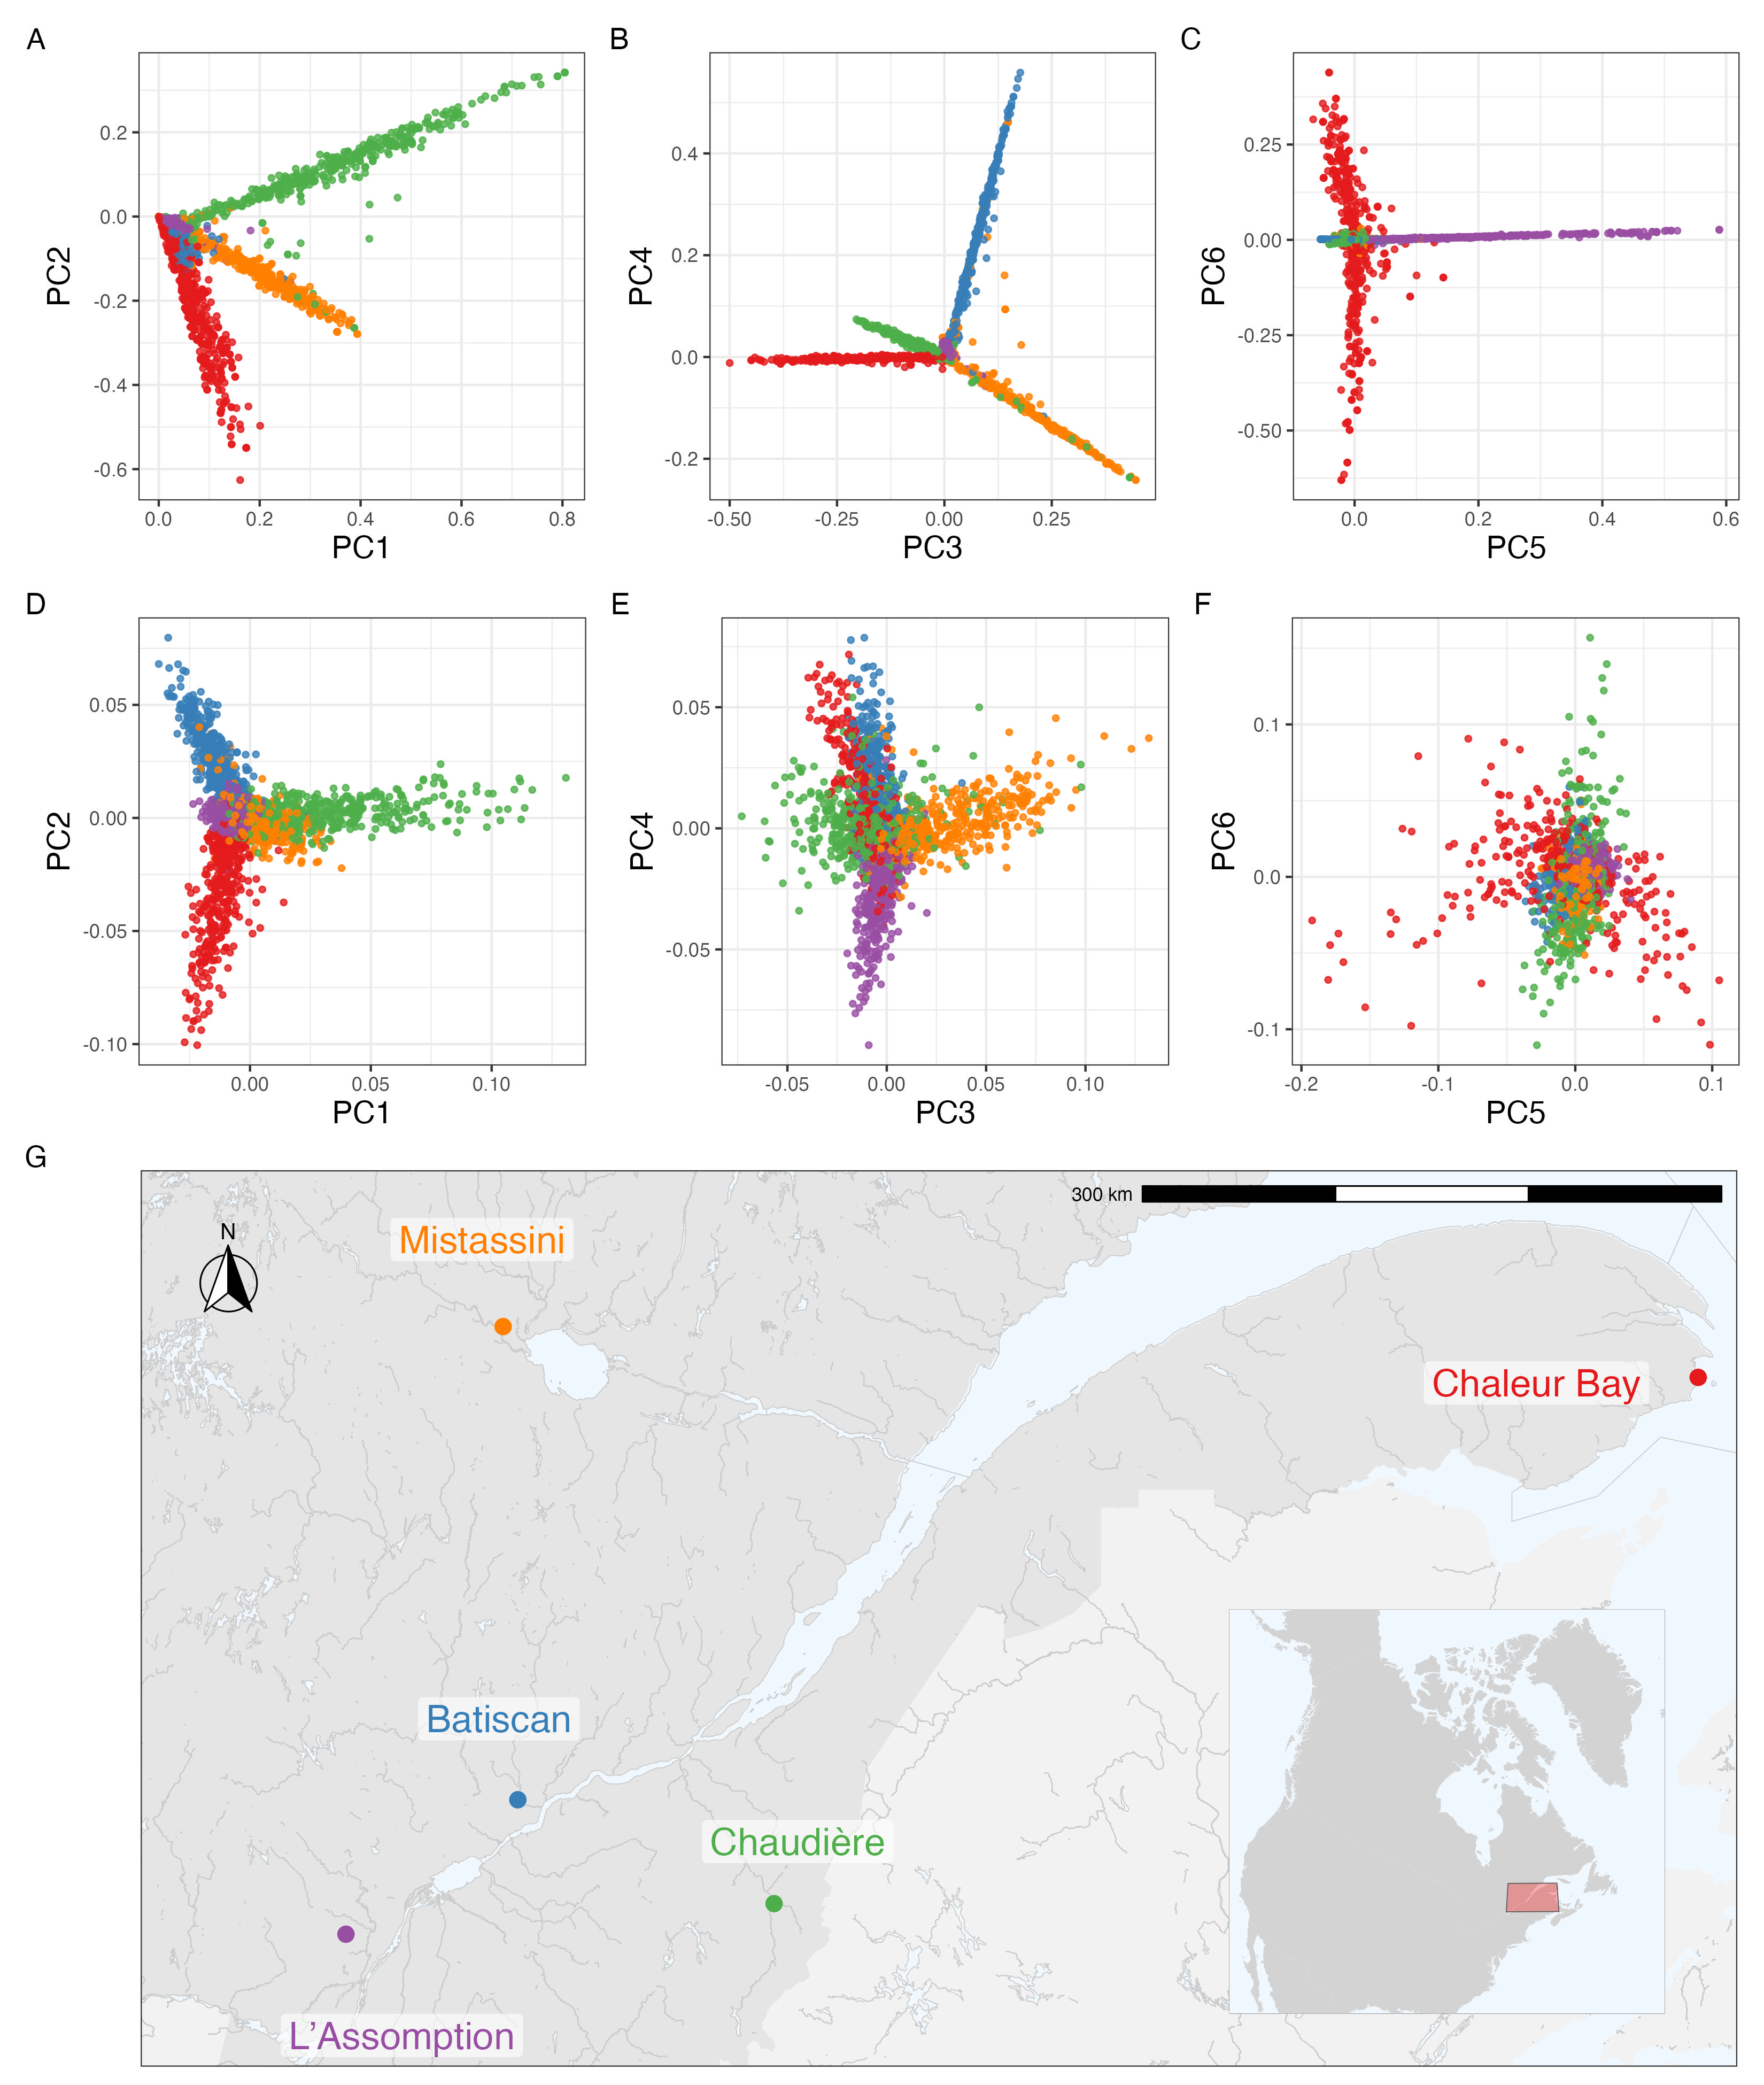
\includegraphics[width = \textwidth]{Figures/map_and_pca_grid4.jpg}
    \caption{Principal components analysis of pedigree and branch GRM of French-Canadian individuals.
    (A-C) The first six principal components of pedigree GRM.
    (D-F) The first six principal components of branch GRM.
    (G) A partial map of Quebec with approximate locations of sampled individuals. \label{fig:PCA_map}}
\end{figure}

% Paragraph on pedigree PCs
The overall population structure according to pedigree and branch PCA
of the 2,321 probands is shown in Figure~\ref{fig:PCA_map}
with noticeable clustering by the five regions.
%
The pedigree PCs show sharp distinctions between individuals from different regions
(Figure~\ref{fig:PCA_map}A-C).
%
Although individuals from each of the regions share a common bottleneck,
over the last four centuries,
each of the regions have drifted in their own unique way
leading to each region pulling a distinct principal component.
%
PCs 1 and 2 show a clear structure between individuals from Chaudière, Chaleur Bay, and Mistassini.
%
PCs 3 and 4 distinguish between individuals of each of the five regions except L'Assomption.
%
PCs 5 and 6 illustrate a clear distinction between L'Assomption and Chaleur Bay.
%
Only a few individuals deviated from the clusters.
\todo[inline]{Luke: are these descendants of migrants?}
\todo[inline]{Gregor: Yes. The great majority of French Canadian ancestry is attributed to French Settlers from four hundred years ago. Most settlers would have arrived in Quebec City, then radiated out from there. Each of the samples regions would have been founded by migrants who descended from these Quebec City founders.}

% Paragraph on branch PCs
The branch PCs also show the population structure (Figure~\ref{fig:PCA_map}D-F),
but there are at least two notable differences compared to pedigree PCs.
%
First, some regions clustered differently with branch PCs than with pedigree PCs.
%
This difference could be because branch PCs are based on the ARG,
which captures deeper ancestry than the pedigree,
however due to the shared bottleneck and pedigree missingness
further research is needed to study the source of these differences.
\todo[inline]{Luke: would any of these changes make sense in the light of known ancestry that is not encoded in pedigree?} 
\todo[inline]{Gregor: I'm not sure I agree with the statement "branch PCs are based on the ARG, which captures deeper ancestry than the pedigree". The ARG is based on the same information as the pedigree, if anything the pedigree has more information that the ARG because of the finite size of the genome.

If anything, I think the differences could be attributed to more noise in the ARG compared to the pedigree. The genome simulations introduce a lot of "noise" (see figure 4) and I think the PCs reflect a similar noise. 

Brieuc and I had previously identified that individuals with shallow pedigrees tend to appear at the origin of the PCA. These "shallow" individuals will be most similar to the simulated founders (EUR from the tennessen OOA model). Even though we removed individuals with very shallow genealogies, I suspect that pedigree missingness could still play a role in influencing the number of individuals near the origin of the PCA -- for both pedigree and ARG relatedness. }
%
Second, branch PCs show more variation than pedigree PCs.
%
This higher variation is partly because we have used one simulated ARG (for one chromosome)
for the branch GRM, leading to a high variance in branch PCs,
but again also because of deeper ancestry encoded in the ARG,
which pedigree does not capture.
% 
\todo[inline]{Brieuc: Confim/check/rewrite this sentence (on the one ARG used for branch GRM}
\todo[inline]{Brieuc: Could we average/sum? ~23 branch GRMs, and run PCA on that and
show that this reduces noise in branch PCs (after the initial submission!?)
Would this be another row in this plot or a plot in supplement?}
%
% When we have computed branch GRM across 23 simulated ARGs (for 23 chromosomes) within the fixed pedigree,
% the variance in corresponding branch PCs decreased (Figure~\ref{fig:PCA_map}G-I / \ref{fig:PCA_map23}).
%
\todo[inline]{Brieuc: Could we show genotype PCA compared to branch PCA in supplement?
(after the initial submission!?)}

\subsubsection{Comparing pedigree and branch GRM}

Comparison of relatedness between 250 French-Canadian individuals shows
a stronger structure with pedigree GRM than with branch GRM (Figure~\ref{fig:grm_heatmap}).
%
The difference between the two GRMs is stark
due to the randomness of genetic inheritance for a single chromosome,
which is not captured by pedigree.
%
\todo[inline]{Brieuc: Could we average/sum? ~23 branch GRMs, and show heatmap on that? (after the initial submission!?)}
% When branch GRM is computed across 23 simulated ARGs (for 23 chromosomes) within the fixed pedigree,
% the similarity between the pedigree and branch GRMs increased (Figure~\ref{fig:grm_heatmap23}).
%
Notably, when individuals have a shallow pedigree
(for example, one sampled individual from Chaleur Bay),
their corresponding pedigree GRM rows and columns have low pedigree relatedness,
while this is not the case with branch relatedness.

\begin{figure}
    \centering
    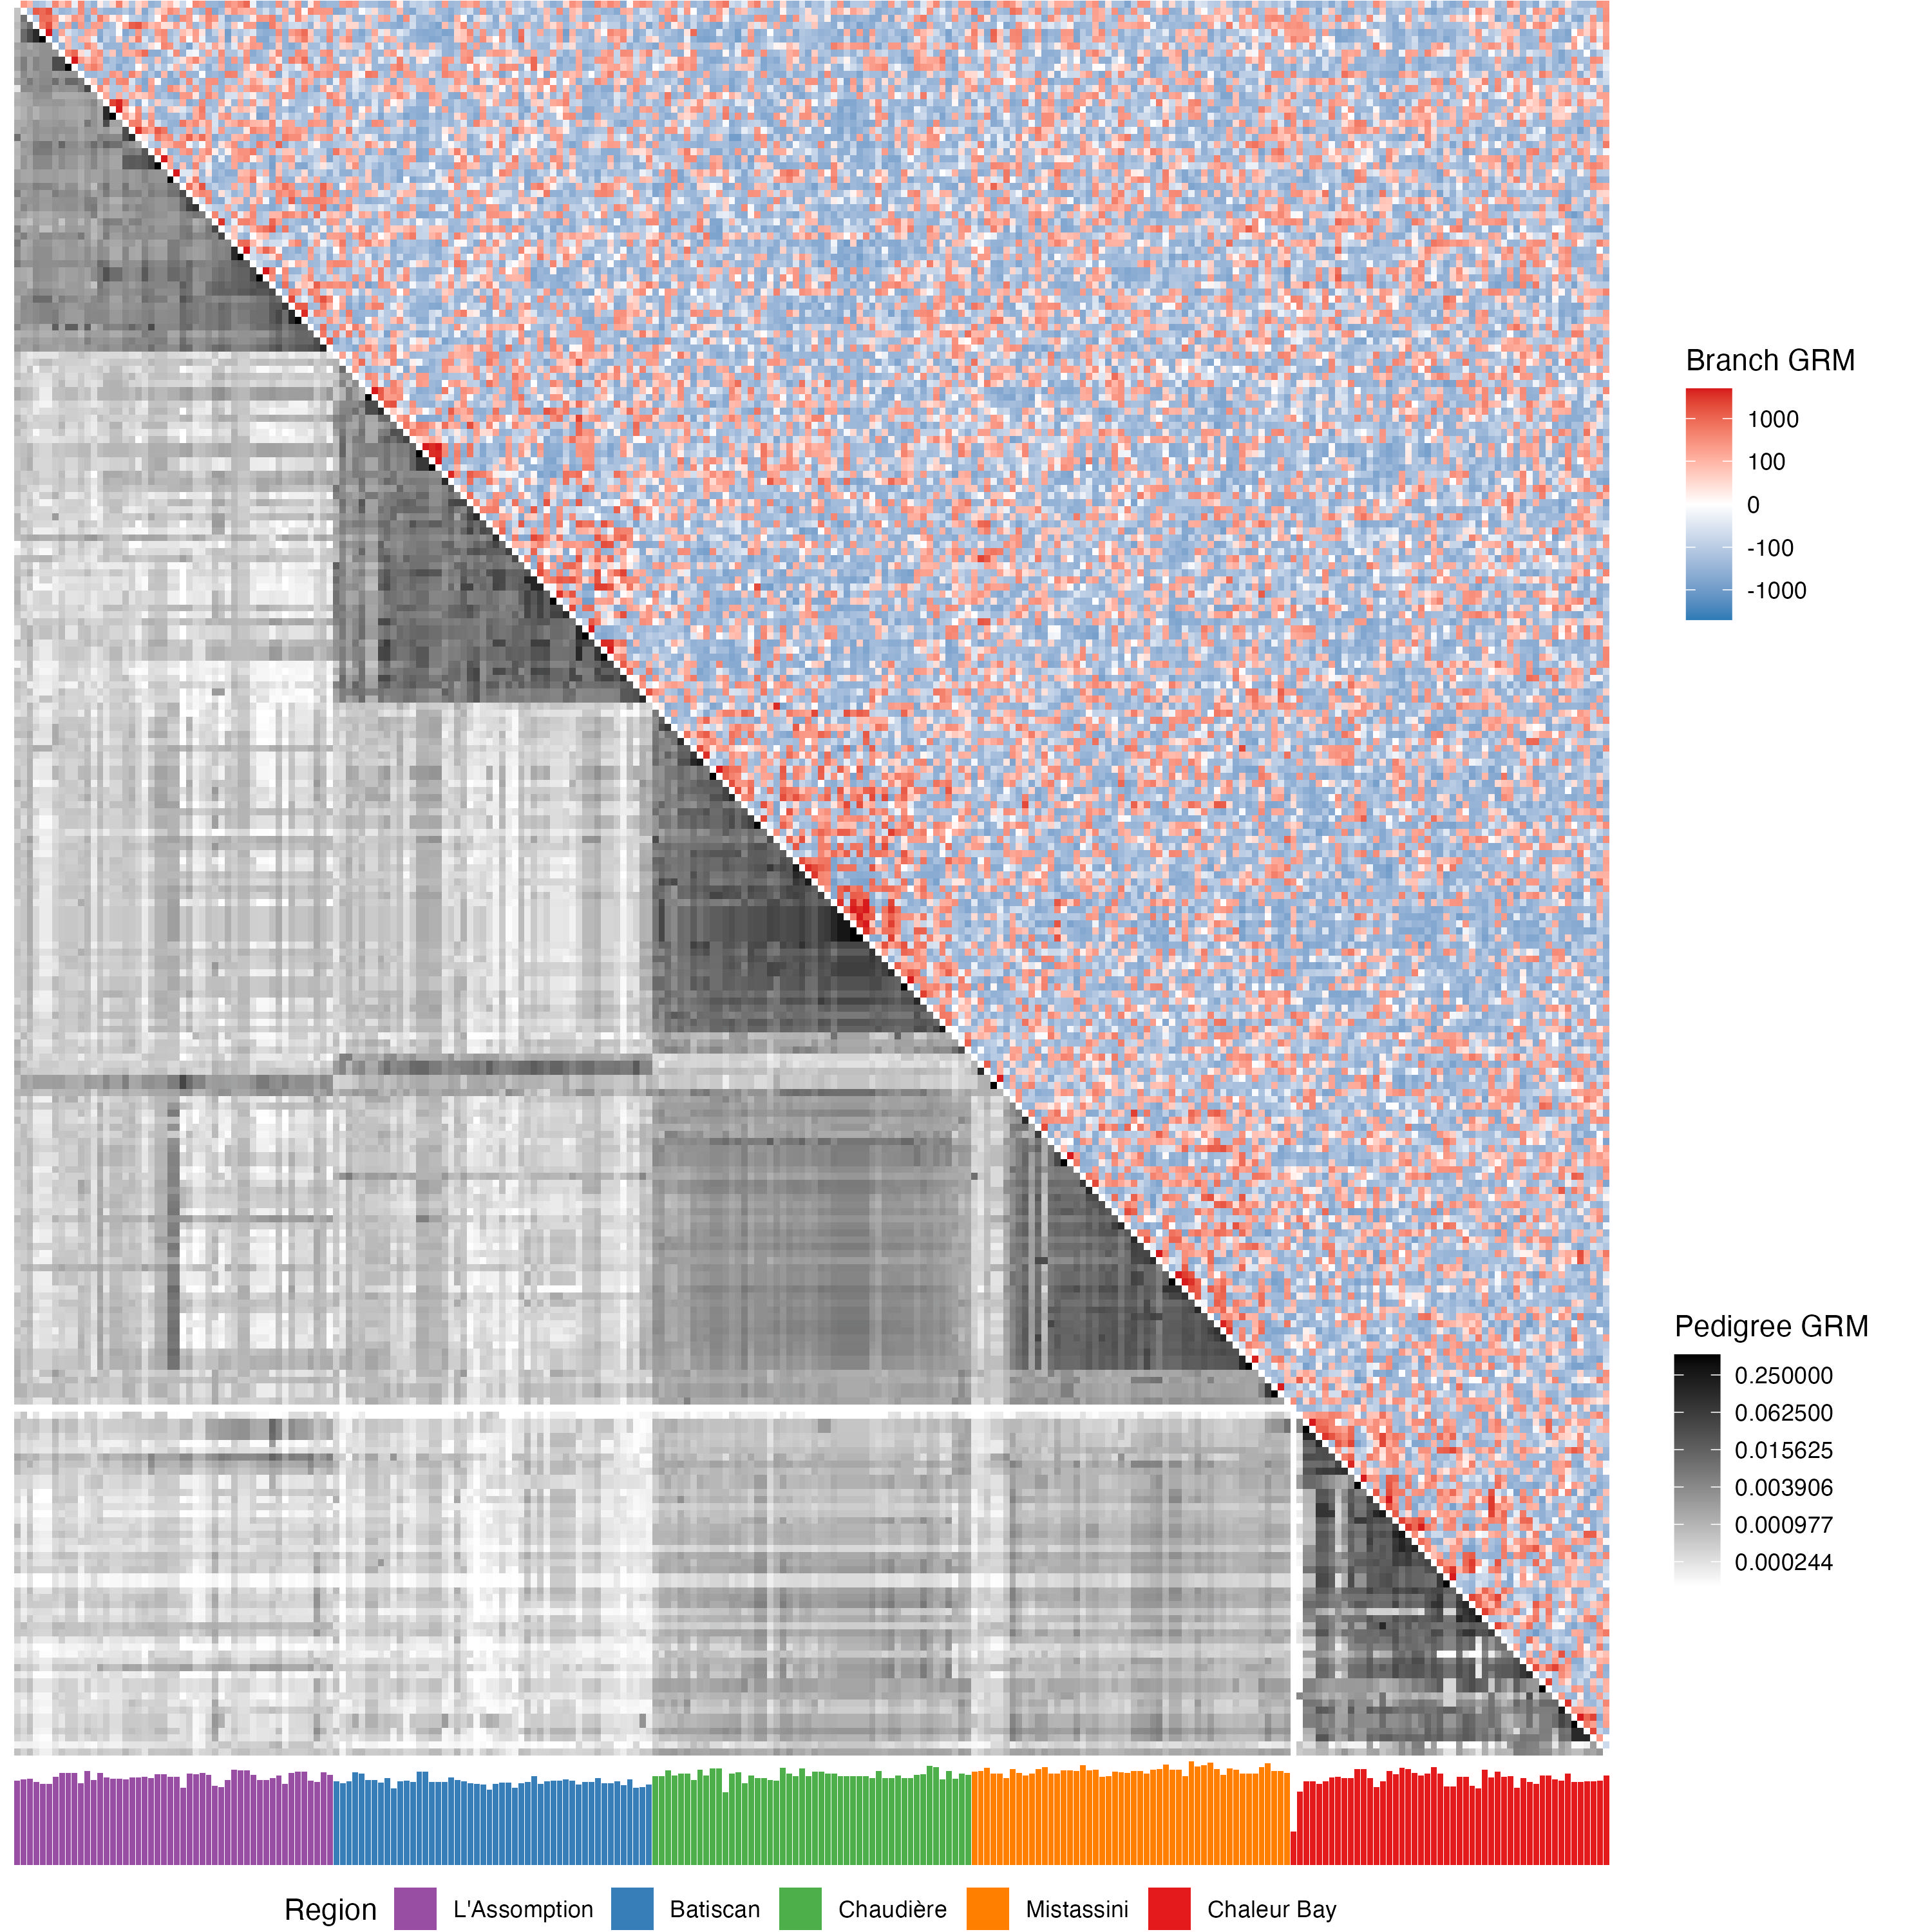
\includegraphics[width=\textwidth]{Figures/Fig4_grm_prm_heatmaps4.jpg}
    \caption{Relatedness between 250 French-Canadian individuals from 5 regions in Quebec.
      Upper-triangle: Heatmap of the branch GRM computed from one ARG (one chromosome).
      Lower-triangle: Heatmap of the pedigree GRM. 
      Bottom: Barplot of the average founder depth in the pedigree for each individual.
      The ordering of individuals is based on region and within region hierarchically on pedigree GRM.
      Because of the log scaling in the heatmap of branch GRM, we used an epsilon of 1e-4 to avoid issues with values close to zero.
    }
    \label{fig:grm_heatmap}
\end{figure}

\subsubsection{Variability in branch GRM within a fixed pedigree}

% Paragraph on main relationship between branch and pedigree relatedness
Next, we explored the variability in branch relatedness across the 100 simulated ARGs
(Figure~\ref{fig:boxplots}).
%
As expected, the branch relatedness increases with pedigree relatedness.
%
Since pedigrees are often shorter than the mean TMRCA,
and so the contribution of branch lengths within the pedigree is small,
a simple approximation of the relationship between the two
can be derived as follows.
%
First, since pedigree relatedness $r_{i,j}$ between a pair of individuals
is the expected proportion of the genome on which the two inherit from
a common ancestral genome within the pedigree,
we expect branch relatedness $C_{i,j}$ to be $r_{i,j} C_0 + (1 - r_{i,j}) C_*$,
where $C_0$ is the average branch relatedness of a genome to itself in pedigree founders,
and $C_*$ is the average branch relatedness of two distinct genomes from the pedigree founders.
%
Since this relatedness is \emph{centered}, we can (very roughly) take
$C_* \approx 0$ and $C_0 \approx A(U,U) - A(U,V)$ (with $U$ and $V$ random individuals).
%
In other words, the average centered branch relatedness
of a typical genome to itself is the total area of edges back to the roots,
minus shared edges between two typical (but different) genomes.
%
Using the relationship~\eqref{eqn:divergence_relatedness},
this is $C_0 \approx D(U,V)/2$.
%
Hence, we expect $\mathbf{B}_{i,j} \approx r_{i,j} T$
where $T$ is the mean TMRCA for two random samples from the population
(computable as one half of branch genetic divergence in \tskit{}).
%
This is shown with a line in Figure~\ref{fig:boxplots},
with $T$ computed from the demographic model used for recapitation of the pedigree.

% Paragraph on variance in branch relatedness compared to pedigree relatedness
However, there is a degree of variability in branch relatedness
between different pairs of individuals with similar pedigree relatedness.
%
While branch relatedness broadly tracks the expected relatedness outlined above,
the median relatedness varies around this value across the range of pedigree relatedness.
%
Moreover, there is substantial variability in branch relatedness within a single pair of individuals.
%
This variability is highest for sibling pairs and decreases with pedigree relatedness.

% Paragraph on summarising branch and ped relatedness
Taken together, these results illustrate that, even in a fixed pedigree,
there can be substantial variation in branch relatedness at one chromosome,
and that the degree of variation varies with respect to pedigree relatedness.
%
We emphasize that these results are obtained from simulations of a single chromosome.
%
We expect the absolute variability to decrease when considering
branch relatedness across the whole genome.

\begin{figure}
    \centering
    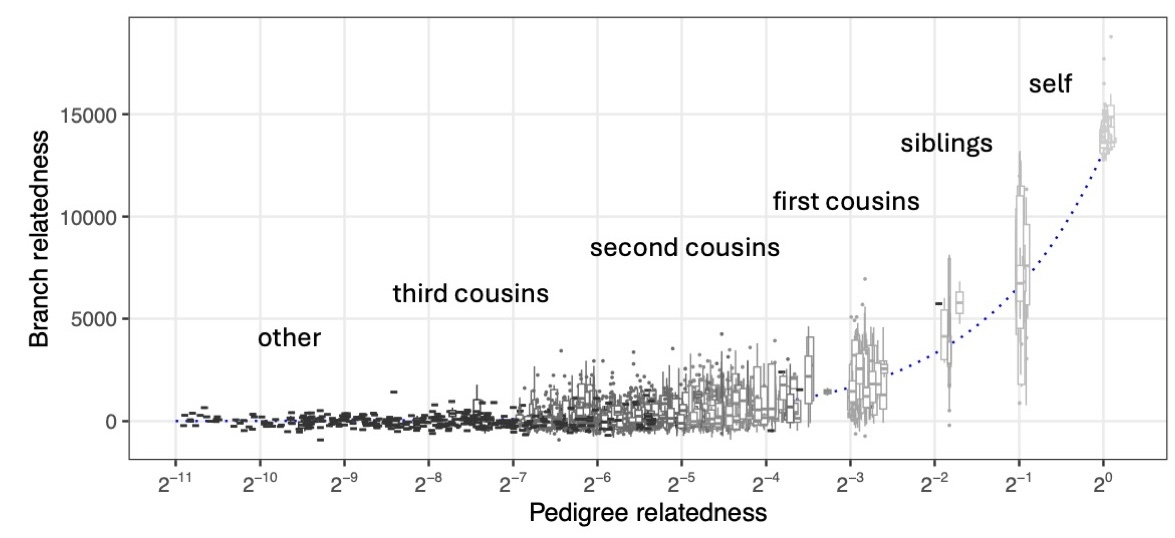
\includegraphics[width=\textwidth]{Figures/Fig5_branch_recap_sim_boxplot_combined_behind2.jpg}
    \caption{Variability in branch relatedness with respect to a fixed pedigree.
    Each box plot corresponds to a pair of individuals with pedigree relatedness
    according to some types of (pedigree) relationships (self, siblings, etc.).
    The box plot for each pair of individuals depicts variation in branch relatedness across 100 ARGs within the fixed pedigree.
    The dotted line indicates the approximate expected branch relatedness,
    which is the pedigree relatedness multiplied by the mean TMRCA among pedigree founders.}
    \label{fig:boxplots}
\end{figure}

% --- EXAMPLE ------------------------------------------------------------

% \subsection{An illustrative example}

% 
\todo[inline]{Update diagram of tree sequence and corresponding notion of relatedness.}
\begin{figure}
    \centering
    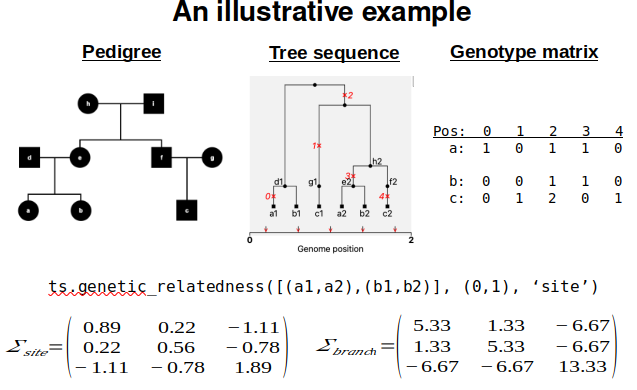
\includegraphics[width=\textwidth]{Figures/ts_gr_example.png}
    \caption{Placeholder for illustrative diagram}
    \label{fig:illustration}
\end{figure}

% \gregor{I think at least one recombination (so we have two local trees) would be nice to have and to connect better to IBD segments.}

% --- GRM computation ----------------------------------------------------

\subsection{Efficient branch GRM-vector products}

% Paragraph on tskit implementation
We now describe algorithms to perform computation of, and with, branch GRM
from a tree sequence encoding of an ARG.
%
These are implemented in the \tskit{} software \citep{ralph2020efficiently, kelleher2024tskit},
a highly performant toolkit for storing, manipulating, and analysing genomes using the tree sequence data structure
\citep{kelleher2016efficient, kelleher2018efficient, wong2023general}.
%
We note that the \eGRM{} package implements the tree-by-tree approach of
\citet{fan2022genealogical} and the \ARGneedlelib{} library implements the
mutation-dropping approach of \citet{zhang2023biobank}.

\subsubsection{Computing branch GRM}

% Paragraph on computing the distance matrix
% Notation debatable! Just sticking in the first thing I thought of.
The fundamental object of interest in this work is the divergence matrix $\mathbf{D}$,
which computes the [precise defition] diversity \todo{Write precise definition}
such that $\mathbf{D}_{i, j}$ is the diversity between samples $i$ and $j$.
%
The algorithm used is straightforward, essentially iterating
over all pairs of samples in each tree along the genome, computing the
time to their MRCA, and updating the corresponding element of $\mathbf{D}$.
%
MRCAs are computed efficiently using the Schieber-Vishkin
algorithm \citep{Schieber1988On} \todo{add Knuth citation!?},
which allows us to compute the MRCA of two nodes in constant time
after an $O(n)$ preprocessing step.
% When searching for Schieber1988On, I found the following paper. Is it useful?
% Simpler O(1) Query Algorithm for Level Ancestors
% https://arxiv.org/html/2207.11954v3
%
Given this, the overall time complexity is $O(n_T n^2)$,
as we need to perform $O(n^2)$ for all $n_T$ trees.
%
It is interesting to note that much more sophisticated
``incremental'' algorithms taking advantage of the differences between
adjacent trees and updating the divergence matrix only when necessary
were much slower in practice than the simple approach outlined above.
%
One possible explanation is that the dominant $O(n^2)$ term here means
that trees never become large enough to justify the more complex
code, and a well-engineered simple approach is faster in practise.

% Paragraph on computing GRM from D
Given $\mathbf{D}$ we can compute the branch GRM in a straightforward manner via:
%
\[
\mathbf{G} = \mbox{do something with}\mathbf{D}
\]
\todo{Complete this paragraph.}

Supplementary Fig~XX compares the \tskit{} implementation of this
algorithm to the \eGRM{} package~\citet{fan2022genealogical}, showing
% JK note: it should, we'll fix this.
that it is significantly faster. 

% and the \ARGneedlelib{} library implements the
% mutation-dropping approach of \citet{zhang2023biobank}.

% % Paragraph on GRM benchmark times
% We found that across a range of settings, our implementation of branch GRM computation,
% \texttt{ts.genetic\_relatedness\_matrix}, outperforms that of the \eGRM{} package
% (Figure~\ref{fig:benchmarking}A,B).
% %
% As expected, the compute time increased with both number of samples and sequence length.
% %
% The relative gap in computation time decreased with the number of sample nodes,
% while remaining stable with the genome sequence length.
% %
% For example, the average time taken to compute the branch GRM
% for $2^9 = 512$ sample nodes was
% 258s for \eGRM{} and 52s for \tsGRM{},
% corresponding to a difference of 3.4 minutes.
% %
% For $2^{12} = 4096$ sample nodes, this difference increased to 11.2 minutes:
% \eGRM{} took on average 86.4 minutes (XYZ seconds) while
% \tsGRM{} took on average 75.2 minutes (XYZ seconds).
% \todo[inline]{Brieuc: This reads very well, but looking at the plot I have to convert all the time, so I suggest adding seconds in brackets.}
% %
% Both implementations reached the memory limit of 4GB
% while computing the GRM for $2^{13}=8192$ sample nodes.

\subsubsection{Computing branch GRM-vector products}

% Paragraph on matvec for branch GRM via simulating gv
Many calculations with GRMs involve matrix-vector products
\citep{colleau2002indirect, colleau2017fast}.
%
As a stepping stone towards a scalable branch GRM-vector product algorithm,
we first present an efficient genetic value simulation algorithm.
%
The notation $m \in_{T_k} n$ means that mutation $m$ is on node $n$ at the $k^{\text{th}}$ tree.
%
We can write the genetic value of sample $s$ as:
%
\begin{align} \label{eqn:genetic_value_trees}
    Z(s) = \sum_k \sum_{n: s\le_{T_k} n} \sum_{m:m \in_{T_k} n} \beta_m
\end{align}
%
given that $\beta_m$ is the effect size of the derived allele due to $m$.
%
Here, we implicitly assume that a child mutation cannot occur at the same site as the parent mutation.

% Paragraph on pushing mutations down the tree
Computing $Z(s)$ can be conceptualized as pushing the mutations down the tree.
%
We can think of the effect size sums as a weight of a node specific to a local tree,
motivating the following notation.
%
\begin{align}
    w_k(n) = \sum_{m: m \in_{T_k} n} \beta_m .
\end{align}
%
This term is similar to the weights in \citet{ralph2020efficiently},
although the resemblance does not play a meaningful role here.
%
Unlike the algorithm in \citet{ralph2020efficiently},
which climbs up the trees from the tips to the root to aggregate the weights of samples,
computing the value~\eqref{eqn:genetic_value_trees} can be conceptualized as
pushing the weights from the root down to the samples at the tips.

% Paragraph on when to push down
The question for an efficient implementation of this idea
is when we should push down $w_k(n)$ for each node $n$.
%
A brute-force strategy is to do this for every tree.
%
However, the sheer number of local trees makes it intractable in large genomes.
%
Efficient tree sequence algorithms leverage the shared tree topology
in adjacent trees to minimize the number of operations.
%
In the following Algorithm~\algorithmref{GVSim},
we only push the weights down when the subtree of the node changes
as we move from left to right.
%
For each node $n$, we have \textit{value} $v(n)$ that collects the genetic effects from above until the subtree changes and
the \textit{index} $l(n)$ storing the last tree index in which $n$ was updated.

% The algorithm
\begin{taocpalg}{GVSim}{Genetic value simulation}
{
    Given a sequence of positions that are recombination breakpoints $b_k$ for $1 \le k \le K$ % TODO: we used b for somehing else before
    along the genome and corresponding sequences of edges to remove ($R_k$) and add ($A_k$) at each position,
    compute the values
    \eqref{eqn:genetic_value_trees} for $1 \le s \le n_S$, as long as all samples are leaves in all trees.
    %
    Let $T$ be the current tree,
    initialize $k = 1$, $l(n)=0$, and $v(n) = 0$ for all $n \in \mathbf{V}$.
}

\algstep{G1.}{Remove edges}{
    For each edge $(c, p) \in R_k$,
    identify the path from $p$ to the root.
    Move from the root to $p$ along the path.
    For each $n$ on the path,
    $v(n) \pluseq \sum_{l=l(n)}^k w_l(n)$ and $l(n)=0$.
    Then,
    $v(d) \pluseq v(n)$ for all children $d$ of $n$ and
    $v(n)=0$.
    Then,
    $v(c) \pluseq \sum_{l=l(c)}^k w_l(c)$ and $l(c)=0$.
    Finally, remove the edge.
}

\algstep{G2.}{Add edges}{
    For each edge $(c, p) \in A_k$,
    identify the path from $p$ to the root.
    Move from the root to $p$ along the path.
    For each $n$ on the path,
    $v(n) \pluseq \sum_{l=l(n)}^k w_l(n)$ and $l(n)=0$.
    Then,
    $v(d) \pluseq v(n)$ for all children $d$ of $n$ and
    $v(n)=0$.
    Then, $l(c)=0$.
    Finally, add the edge.
}

\algstep{G3.}{Iteration}{
    If $k < N$,
    set $k = k + 1$ and return to \algorithmref{\textbf{V1}}.
    Otherwise, set $z_s = v(s)$ for $1 \le s \le n_S$ and finish.
}

\end{taocpalg}

% Paragraph on describing the algorithm
The algorithm only adds the genetic values from above to its child when the subtree changes.
%
This saves the number of operations compared to pushing things down for every tree
because most edges remain the same between close trees.
%
Next, it ensures that a mutation's effect is passed down to the correct samples
because the genetic effects that nodes have accumulated
are passed down just before the samples beneath them change due to an edge insertion or deletion.
%
After passing the previously accumulated genetic effects,
$v(n)$ is set to zero and starts collecting genetic values for the new set of samples.
%
This is why we have to track $l(\cdot)$ to remember the last time the node was updated,
as we should only send genetic values that has not yet been passed to the child.
%
Hence, we can say that the algorithm \textit{lazily} passes
the genetic values from the root to the tips only when it is necessary;
when the samples below a node changes.
%
In other words, sending genetic values from above to below before the subtree change is redundant,
and not doing so when the subtree changes will pass the values to the wrong samples.

% Paragraph on changing the algo to matvec
A slight modification of the algorithm can multiply the GRM to a vector.
%
Suppose that $\mathbf{C}_{s,t}$ is an uncentered branch relatedness between
sampled genomes $s$ and $t$ as computed from the trees, that is,
the sum of the areas of all branches in all trees that are ancestral to both $s$ and $t$.
%
% TODO: we used b for somehing else before
\begin{align} \label{defn:pairwise_relatedness}
    \mathbf{C}_{s,t} = \sum_k (b_k - b_{k-1}) \sum_{n: s,t \le_{T_k} n} \ell_{T_k}(n) % TODO: what is \ell_{T_k} here?
\end{align}
%
For a given vector $\mathbf{w}$, we'd like to compute the matrix-vector product $\mathbf{C}\mathbf{w}$.
%
% TODO: we used b for somehing else before
Suppose that $b_k$ ($k=0,\ldots,K$) are the recombination breakpoints on the genome
including the start and end of the genome (the genome is a closed interval $[b_0, b_K]$).
%
Suppose that the $k^{\text{th}}$ tree $T_k$ extends over a span $b_k - b_{k-1}$ along the genome,
that the length of the edge (in units of time) above node $n$ in $T_k$ is $\ell_{T_k}(n) = t_{p(n)}-t_n$,
where $p(n)$ is the parent node of $n$.
%
The partial ordering $\le_T$ of nodes are induced by the tree that older nodes are larger than the younger nodes.

% Paragraph on computing the matrix-vector product
The $s^{\text{th}}$ element of the matrix-vector product $\mathbf{C}\mathbf{w}$ is:
%
\begin{align} \label{eq:similar_ralph2020}
    \begin{aligned}
        (\mathbf{C}\mathbf{w})_s &=
        \sum_t \mathbf{C}_{s,t} w_t \\
        &=
        \sum_t
        \left(
            \sum_k (b_k - b_{k-1}) \sum_{n: s,t \le_{T_k} n} \ell_k(n)
        \right) {w}_t \\
        &=
        \sum_k (b_k - b_{k-1})
        \sum_t
        \sum_{n: s,t \le_{T_k} n} \ell_{T_k}(n) {w}_t \\
        &=
        \sum_k (b_k - b_{k-1})
        \sum_{n: s\le_{T_k} n} \ell_{T_k}(n)
        \sum_{t:t \le_{T_k} n} {w}_t \\
        &=
        \sum_k (b_k - b_{k-1})
        \sum_{n: s\le_{T_k} n} \ell_{T_k}(n) w_k(n)
    \end{aligned}
\end{align}
%
The new variable $w_k(n)$ is the sum of sample weights below $n$ in tree $T_k$:
%
\begin{align}
    w_k(n) = \sum_{t:t \le_{T_k} n} {w}_t ,
\end{align}
%
which is a familiar term from \citet{ralph2020efficiently}.
%
Although a single entry of $\mathbf{C}\mathbf{w}$ could be computed efficiently
from the algorithm in \citet{ralph2020efficiently},
it doesn't scale well because it would require separate set of weights for each entry of the vector.

% Paragraph on efficient way of computing the matrix-vector product
We present an efficient algorithm for computing the entire matrix-vector product.
%
The general idea is simple: as we move left-to-right along the tree sequence,
we keep track of two things for each node $n$:
the \textit{weight} $w(n)$ of the node in the current tree ($w_k(n)$ above) and
the \textit{value} $v(n)$ of the haplotype carried by $n$,
which will contribute to all descendants of $n$ (we will explain the role of $v(\cdot)$ in detail shortly).
%
Additionally, we keep track of the last \textit{position} $x(n)$ in which the node was updated.
%
As we move along the genome, we update any nodes ancestral to any changes in the tree:
all other nodes are the roots of unchanged subtrees and hence remains unchanged.
%
As seen above, each branch contributes to potentially many entries in the output vector,
so by accumulating values of haplotypes, we reduce the amount of necessary work.

% The algorithm
\begin{taocpalg}{bGRM-vec}{Branch GRM times a vector}
{
    Given a sequence of positions that are recombination breakpoints $b_k$ for $1 \le k \le K$
    along the genome and corresponding sequences of edges to remove ($R_k$) and add ($A_k$) at each position,
    compute the values
    $y_s=\sum_t\mathbf{C}_{st} w_t$ for $1 \le s \le n_S$, as long as all samples are leaves in all trees.
    %
    Let $T$ be the current tree,
    $\ell_T(n) = t_{p(n)} - t_n$ be the length of the branch above $n$ in $T$ (or zero, if $n$ has no parent),
    initialize $k = 1$, $x(n) = 0$, and $v(n) = 0$ for all $n \in \mathbf{V}$.
    Set $w(s) = w_s$ for each sample $s$, and $w(n)=0$ for all other nodes.
    At all times, define
    $z(n) = \ell_{T_k}(n) (b_k - x(n)) $ where $T_k$ is the current tree.
}

\algstep{V1.}{Remove edges}{
    For each edge $(c, p) \in R_k$,
    identify the path from $p$ to the root.
    Move from the root to $p$ along the path.
    For each $n$ on the path,
    $v(n) \pluseq z(n)w(n)$ and
    $x(n)=b_k$.
    Then,
    $v(d) \pluseq v(n)$ for all children $d$ of $n$ and
    $v(n)=0$.
    Then,
    $v(c) \pluseq z(c)w(c)$ and set $x(c)=b_k$.
    Move from $p$ to the root along the path.
    For each $n$ on the path,
    $w(n) \minuseq w(c)$.
    Finally, remove the edge.
}

\algstep{V2.}{Add edges}{
    For each edge $(c, p) \in A_k$,
    identify the path from $p$ to the root.
    Move from the root to $p$ along the path.
    For each $n$ on the path,
    $v(n) \pluseq z(n)w(n)$ and
    $x(n)=b_k$.
    Then,
    $v(d) \pluseq v(n)$ for all children $d$ of $n$ and
    $v(n)=0$.
    Then,
    $x(c)=b_k$.
    Move from $p$ to the root along the path.
    For each $n$ on the path,
    $w(n) \pluseq w(c)$.
    Finally, add the edge.
}

\algstep{V3.}{Iteration}{
    If $k < N$,
    set $k = k + 1$ and return to \algorithmref{\textbf{V1}}.
    Otherwise, set $y_s = v(s)$ for $1 \le s \le n_S$ and finish.
}

\end{taocpalg}

% Paragraph on describing the matvec algorithm
We can see from equation~\eqref{eq:similar_ralph2020} that $\mathbf{C}\mathbf{w}$ is
a sum of the contributions $\ell_{T_k}(n)w_k(n)$ of nodes specific to local trees.
%
Adding these contributions directly to the entries of $\mathbf{C}\mathbf{w}$ is
inefficient due to the sheer number of node and sample pairs.
%
We can mitigate this by pushing down the contribution of the nodes only to their adjacent child nodes at a time,
in the hope that the contributions will be passed to the correct samples corresponding to the entries of $\mathbf{C}\mathbf{w}$.
%
This is because the local connection between the nodes is extremely sparse in the tree sequence.
The role of value $v(\cdot)$ is precisely to deliver the contributions correctly downwards the trees.
%
For each tree $T_k$, we want to ensure that $n$'s contribution is passed down only to
the samples $s$ such that $s \le_{T_k} n$.
%
A straightforward way is to pass down the contributions at every position $k$.
%
Notice that the samples below a node do not change until the subtree beneath it changes.
%
This change is triggered by edge insertions and deletions happening below the edge,
so we wait until the change happens.
%
Each node accumulates the contributions that are passed down from above
until an edge below it is added or removed.
%
This contribution is stored in $v(n)$ and passed down to the child nodes of $n$ when the subtree changes.
%
This corresponds to the operations in $\mathbf{V1}$ and $\mathbf{V2}$
that happen along the path from the root to $p$.
%
After passing down $v(n)$, it is set to $0$ and $x(n)$ is set to $b_k$ (the current position).
%
Then, $v(n)$ repeats to accumulate the contributions from above, including itself,
for the newly updated set of samples.
%
Lastly, we add or subtract the weights of $c$ from the nodes above similarly to
the algorithm in \citet{ralph2020efficiently} to keep the weights up-to-date.

% Paragraph on the efficiency of the algorithm
The algorithm is efficient because the operations occur locally between adjacent nodes in the tree sequence.
%
We can also see that the nodes in the path from the inserted/deleted edge to the root are
modified to keep the computation minimal.
%
It passes the contributions $\ell_{T_k}(n)w_k(n)$ correctly because
$v(\cdot)$ is passed down whenever the subtree changes.
%
From this point of view, we can interpret $v(\cdot)$ as the sum of contributions that $n$ inherited from above,
but had not yet has been sent to the nodes and samples below in the previous trees.

% --- PCA ----------------------------------------------------------------

\subsubsection{Branch PCA}

We found the principal components (PCs) of the branch GRM
using a randomized singular value decomposition \citep{halko2011findingstructure},
a method that can find the
eigenvectors of a matrix that is only implicitly defined through a matrix-vector multiplication.
Algorithm~\algorithmref{rPCA} explains this process.

\begin{taocpalg}{rPCA}{Randomized PCA of branch GRM}
{
    Let $\mathbf{G}$ be the branch GRM for $n_I$ individuals,
    let $k$ be the desired number of PCs, and $q$ the number of iterations.
    Multiplying $\mathbf{G}$ with a vector is done by Algorithm~\algorithmref{\textbf{bGRM-vec}}.
}

\algstep{P1.}{Range estimation}{
    Sample a random matrix $\boldsymbol{\Omega} \in \mathbb{R}^{n_I \times k}$ in which the entries are independent standard normal variables.
    Obtain a basis matrix $\mathbf{Q} \in \mathbb{R}^{n_I \times k}$ by applying QR decomposition to $\mathbf{G}\boldsymbol{\Omega}$.
    Repeat $q$ times, updating the basis matrix $\mathbf{Q}$
    by applying QR decomposition to $\mathbf{G}\mathbf{Q}$,
    where $\mathbf{Q}$ is from the previous iteration.
}

\algstep{P2.}{Small singular value decomposition}{
    Compute $\mathbf{W} = \mathbf{Q}^\intercal \mathbf{G}$ and obtain
    the singular vector $\mathbf{U} \in \mathbb{R}^{k \times k}$
    by exact singular value decomposition of $\mathbf{W}$.
    Then the columns of $\mathbf{Q}\mathbf{U} \in \mathbb{R}^{n \times k}$
    contain the desired PCs of the branch GRM $\mathbf{G}$.
}

The algorithm has two advantages over directly applying the exact singular value decomposition to the full matrix.
%
It needs less time and memory because the $n_I \times n_I$ branch GRM is never computed nor stored.
%
The algorithm extracts the relevant information through
the efficient matrix-vector product Algorithm~\algorithmref{bGRM-vec}.
%
Secondly, the exact singular value decomposition is applied to an $n_I \times k$ matrix,
where $k$ is much smaller than $n_I$.
%
This reduces the amount of computation considerably.

\end{taocpalg}


\begin{figure}
    \centering
    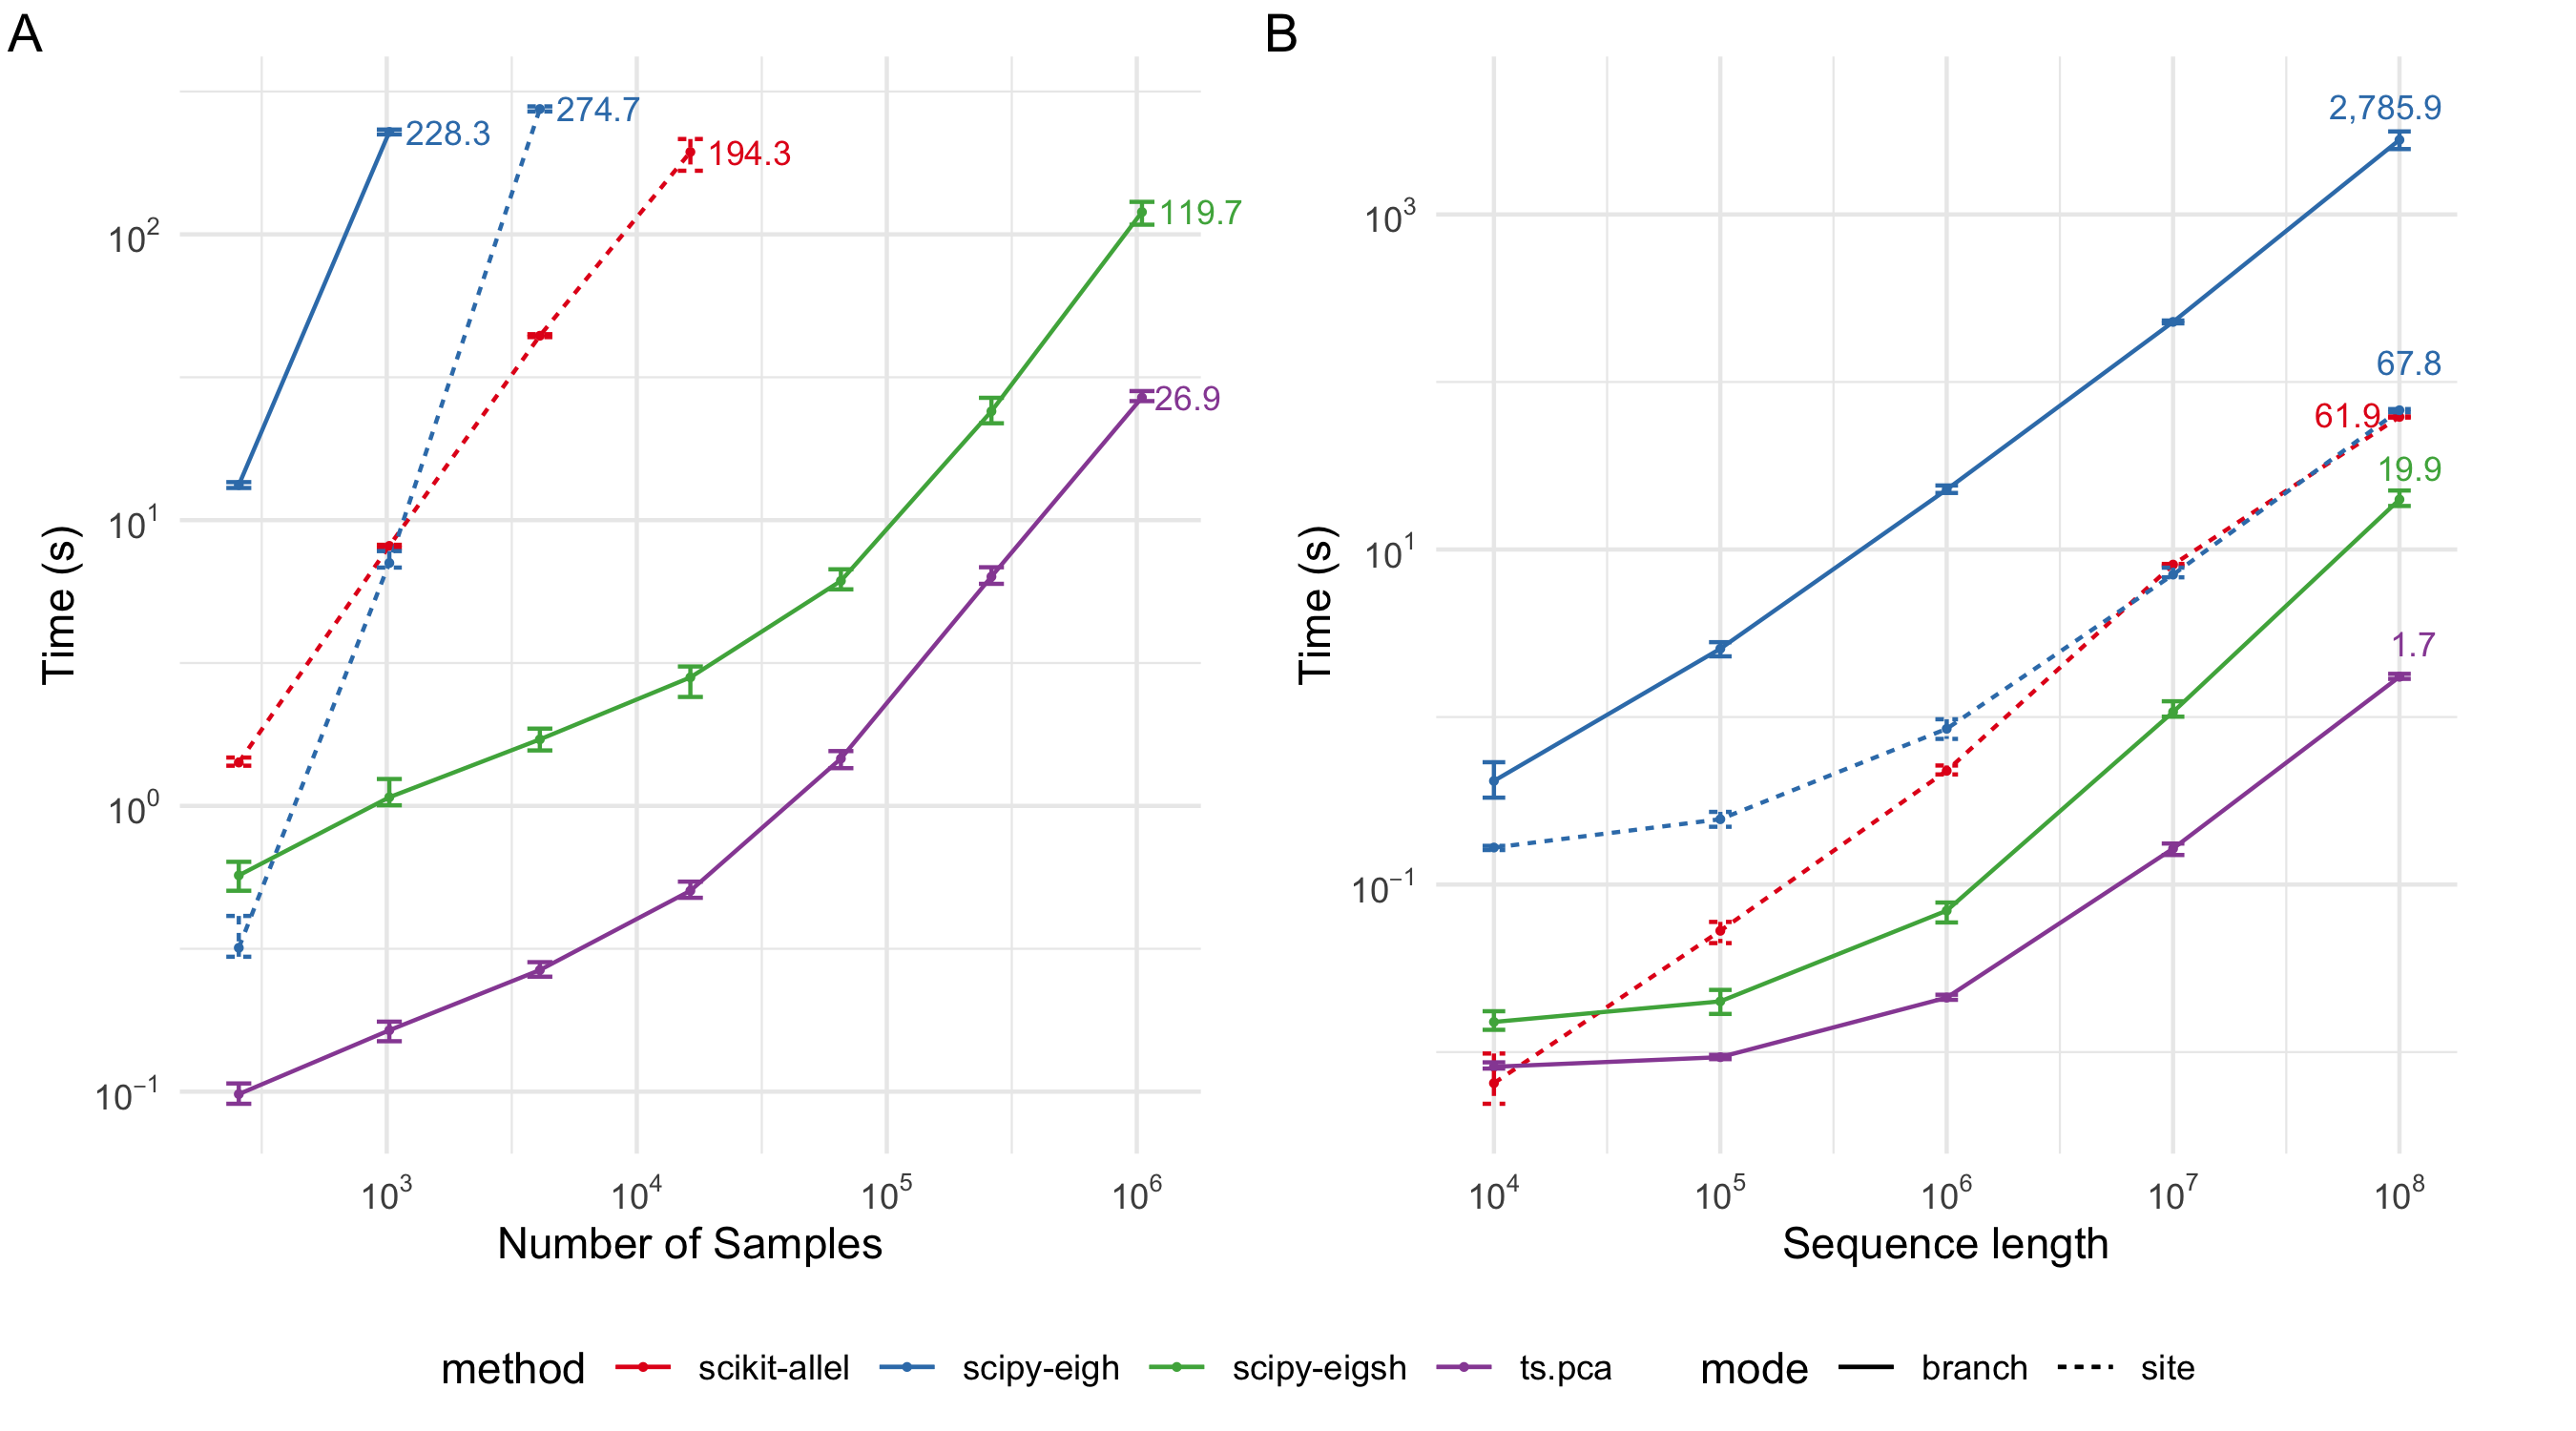
\includegraphics[width=\textwidth]{Figures/Fig2_benchmarking_plot.png}
    \label{fig:benchmarking}
    \caption{Time efficiency of different implementations of branch GRM and PCA computations.
    Each dot corresponds to the average time taken across ten simulations with different random seeds.
    Error bars represent the range in time taken across the ten simulations.
    (A) Branch GRM computation with genome sequence length fixed at $10^{7}$ and varying the number of samples.
    (B) Branch GRM computation with number of sample nodes fixed at $2^{10}$ and varying genome sequence length.
    (C) PCA with genome sequence length fixed at $10^{7}$ and varying the number of samples.
    (D) PCA with number of sample nodes fixed at $2^{10}$ and varying genome sequence length.
    Branch mode refers to branch GRM and site mode refers to genotype GRM.}
\end{figure}
\todo[inline]{Brieuc: Can you ensure the labels are shown in Fig2C for all lines (blue and red don't have them)?
Or was this "omission" intentional"? Maybe also round-off the decimal digits.}


The efficiency of the branch-PCA algorithm (and the underlying GRM-vector
multiplication algorithm is illustrated in Fig~\ref{fig:benchmarking}. 
[DESCRIPTION OF WHAT WE SEE].
See Methods for details of the benchmarking methodology.


% Paragraph on PCA benchmark times
For PCA, we observed significant benefits from using implementations
that avoided the storage of the GRM or genotype matrix in memory,
particularly for larger numbers of samples (Figure~\ref{fig:benchmarking}C,D).
%
Notably, \tsGRM{} failed due to memory limits
when computing the branch GRM for $2^{12} = 4096$ sample nodes and
when computing the genotype (site) GRM for $2^{14} = 16384$ sample nodes.
\todo[inline]{We should mention in M\&M that \tsGRM{} can do site version too!
or just somewhere (discussion - but say that we ideally want to work with branches!?)}
%
Implementation of randomised PCA on genotype matrix in \scikitallel{}
failed due to memory limits for $2^{16} = 65536$ sample nodes.
%
Notwithstanding, the implementations that relied solely on
direct matrix-vector computations using \tskit{} were substantially more efficient.
%
Specifically, both \tsPCA{} and \eigsh{} from \scipy{} using \tsGRw{}
as a linear operator were able to scale to $2^{20} = 1,048,576$ samples.
%
The native implementation of \tsPCA{} consistently outperformed \eigsh{},
with the relative difference remaining reasonably stable with the number of samples,
and increasing with sequence length.
%
The difference in absolute compute time increased with both sample size and sequence length.
\todo[inline]{Brieuc: Lookingh at the plot C, I don't see this - the difference is becoming smaller there;
but the difference is growing in plot D. Revise the text or plot?}
%
For example, \tsPCA{} took on average
0.27s for $2^{12} = 4,096$ samples and
26.9s for $2^{20} = 1,048,576$ samples,
while \eigsh{} took
  1.7s for $2^{12} = 4,096$ samples and
119.7s for $2^{20} = 1,048,576$ samples.
%
This difference primarily reflects the differences in the underlying algorithms used for PCA:
\tsPCA{} uses randomised singular value decomposition while \eigsh{} uses
\todo[inline]{mention what algorithm is used in eigsh - full or truncated eigen or svd? Should we move this sentence in dicsussion instead?}


\section{Methods}


% --- Application --------------------------------------------------------

\subsection{French-Canadian pedigree}

% Paragraph on the French-Canadian pedigree
To demonstrate the similarities and differences between pedigree and branch relatedness, we performed a range of analyses on a subset of an extended pedigree of French-Canadian individuals from the BALSAC project \citep{vezina2020overview}.
%
Spanning over 400 years, this pedigree is compiled from over 4.5 million parish records across Quebec.
%
In this paper, we restricted our analyses to five regions,
each containing five neighboring parishes (Table~\ref{tab:parishes}).
%
Using the migratory patterns from \citet{andersontrocme2023genes} as a reference,
we identified five distinct regions and sampled individuals from parishes within each region 
to minimize excessive relatedness within each sampling unit 
while also mitigating the risk of de-anonymization.
%
Our data access agreements with BALSAC dictated that we use parish records of more than one hundred years old
(before 1924) to publish their metadata and summary statistics.
%
As a result, the pedigree used in this study contains ascending genealogy for
500 randomly chosen contemporary individuals from each of the five regions,
with individuals sampled across the five selected parishes per region.

% Paragraph on filtering individuals
The sub-pedigree obtained from the selected five regions, each containing five parishes,
consisted of 61,490 individuals, including 2,321 probands.
%
A subset of the probands exhibited a low depth of pedigree,
reflecting an incomplete pedigree.
%
To ensure meaningful comparisons, we computed the maximum pedigree depth
for each individual and derived an average depth metric.
%
A total of 48 probands with an average depth of less than 3 were excluded
due to their shallow pedigree.
%
After this filtering step, a total of 2,273 probands were retained for downstream analyses.

\begin{table}
  \centering
  \caption{Selected regions and parishes from the BALSAC French-Canadian Pedigree}
  \renewcommand{\arraystretch}{1.2}
  \resizebox{\textwidth}{!}{%
    \begin{tabular}{|l|p{10cm}|c|}
      \hline
      Region & Parishes & Approximate location \\
      \hline
      Chaleur Bay & St Michel, St François De Sales, St Georges De Malbaie, St Pierre De Malbaie, and St Joseph & 48.5222, -64.2156 \\
      Batiscan & Ste Geneviève De Batiscan, St Luc De Vincennes, St Narcisse, and St Stanislas & 46.5324, -72.3398 \\
      Chaudière & St Georges, St Benoit Labre, St Philibert, St Come, and St Martin De Tours & 46.1184, -70.6691 \\
      L’Assomption & St Jacques, St Alexis, Ste Marie Salomée, and St Esprit & 45.9483, -73.5702 \\
      Mistassini & St Félicien, St Méthode, Notre Dame De La Dore, St Cyrille, and Ste Lucie & 48.6399, -72.4543 \\
      \hline
    \end{tabular}
  }
  \label{tab:parishes}
\end{table}

% Paragraph on pedigree stats and simulated ARGs
We computed pedigree and branch GRM between individuals of interest.
%
Pedigree GRM was computed after
\citet{lange1992calculation} and \citet{colleau2002indirect}.
%
Branch GRM was calculated from an ARG
obtained with the simulation based on pedigree and ancestry
described in \citet{andersontrocme2023genes}.
%
In short, this simulation uses \msprime{} \citep{baumdicker2022efficient} 
for a backward in time simulation in two stages.
%
First, it samples chromosome inheritance through the fixed pedigree
to obtain an ARG within the pedigree.
%
Second, it further samples chromosome inheritance through the assumed demographic model
to recapitate the ARG from the first stage.
%
We elected to simulate only the complete human chromosome 3 due to its large size
while reducing the overall computational cost of our study.
%
To study the stochastic variation in recombination and coalescence events within the pedigree,
we simulated 100 replicates of an ARG for the chromosome using different random seeds.
%
This approach allowed us to assess the variance in branch GRM
while maintaining consistency with the underlying pedigree.

% Paragraph on pedigree and branch PCA
To explore the overall population structure within the pedigree and the simulated tree sequences,
we performed PCA on the set of 2,273 probands.
%
For pedigree PCA, we first computed the pedigree GRM
among the probands and then eigen-decomposed the GRM using
\texttt{eigh} function from \scipy{} \citep{Virtanen2020SciPy}.
%
For branch PCA, to avoid undue influence of large, low-recombination regions,
we first remapped genomic coordinates from base pairs to genetic distance,
using the HapMap II genetic map provided by \texttt{stdpopsim} \citep{adrion2020stdpopsim}.
%
We then used Algorithm~\algorithmref{rPCA} to compute the first six PCs.

% Paragraph on comparing relatedness
To compare pedigree and branch relatedness for specific pairwise relationships,
we focused our attention on a subset of the 2,273 probands.
%
Specifically, we randomly sampled one parish per region and
subsampled at least five siblings, first cousins, second cousins, and third cousins from each parish.
%
We then subsampled additional individuals from each parish
to obtain a total of 50 individuals per parish.
%
With these 250 individuals, we computed the pedigree GRM and a branch GRM
for each of the 100 simulated ARGs.

% Paragraph in one vs many ARGs/chromosomes and code
%In results, we either show outputs based on branch GRM for chromosome 3.
%
% The code for performing these analyses and the simulation studies %is available at \url{https://github.com/brieuclehmann/genome_simulations/tree/brieuc}.


% --- Benchmarks ---------------------------------------------------------

\subsection{Benchmark simulations}

We assess the computational efficiency of our implementations for branch GRM and PCA,
with simulations, recording the time for calculations for a range of tree sequences.
%
We simulated the tree sequences with \texttt{msprime} \citep{baumdicker2022efficient},
and varied either the genome sequence or the number of sample nodes (=haploid individuals).
%
All computations were carried out on a single CPU with 4GB of RAM.

\subsubsection{Branch GRM}

We compared \tsGRM{} for computing the branch GRM to
the implementation in the \eGRM{} package \citep{fan2022genealogical}.
%
The default values for simulations parameters were $10^{7}$ for the genome sequence length,
$2^{10}$ for the number of samples, and effective population size of $10^4$.
%
We then varied
genome sequence length from $(10^{4}, 10^{5}, 10^{6}, 10^{7}, 10^{8})$ and
the number of samples from $(2^7, 2^8, 2^9, 2^{10}, 2^{11}, 2^{12})$,
each one at a time.
%
For each simulation setting, we generated 10 tree sequences with different random seeds and
reported the average time taken to compute the GRM with each implementation.

\subsubsection{Branch PCA}

We assessed our branch PCA Algorithm~\algorithmref{rPCA} against a number of comparators
using \scipy{} \citep{Virtanen2020SciPy} and \scikitallel{} \citep{Miles2024scikit}:
%
\begin{itemize}
    \item Calculating branch GRM using \tsGRM{} followed by eigenanalysis using \eigh{} function from \scipy{}.
    \item Eigenanalysis of branch GRM using \eigsh{} function from \scipy{} using the implicit matrix-vector product Algorithm~\algorithmref{V} as a linear operator.
    \item Calculating genotype GRM using equation~\eqref{eqn:grm} followed by eigenanalysis using \eigh{} function from \scipy{}.
    \item Randomized PCA of genotype matrix using \texttt{randomized\_pca} function from \scikitallel{}.
\end{itemize}
%
We used the same simulations as for the branch GRM computation benchmark,
but explored larger sample sizes, ranging across $(2^8, 2^{10}, 2^{12}, 2^{14}, 2^{16}, 2^{18}, 2^{20})$.
%
For each simulation setting, we generated 10 tree sequences with different random seeds and
reported the average time for PCA with each implementation.



\section{Discussion}


% - ARGs and tree sequences

Recent advances in ARG-based inference have generated significant interest in leveraging ARG-based methods for genetic analyses. In this paper, we examine the relationship between different definitions of genetic relatedness, presenting a unifying framework that connects these concepts through a trait-centric perspective. While relatedness metrics have numerous downstream applications, we expect this perspective to be particularly impactful in phenotypic analyses, such as accounting for population structure in genome-wide association studies and improving genomic prediction, including polygenic scoring.

% - branch relatedness and branch GRM

\todo[inline]{Cite genetic vs genealogical/pedigree ancestors papers and why branch GRM can be more variable than pedigree GRM even when we do it across chromosomes - see results}

% TODO: discuss our variance in branch GRM and Fan et al. vGRM

% \paragraph{uses of relatedness}
% \begin{itemize}
%     \item summary of whole-genome genetic relatedness in a single number
%     \item visualisation, say via PCA
%     \item ontrolling for population "structure" and associated environmental effects in genome-wide association studies ("indirect" use)
%     \item "direct" use in genome-wide association studies and genomic prediction
% \end{itemize}

% - Efficient branch GRM-vector products 
% - Branch PCA

This paper also introduces new algorithms to efficiently perform branch-based relatedness computations. Our approach to computing the branch-based GRM is similar to the algorithm for pedigree-based GRM \citep{emik1949systematic, cruden1949computation, henderson1976simple} in that the algorithm traverses the tree sequence to calculate the GRM for the chosen samples. Additionally, we develop a method for performing matrix-vector product calculations with the branch-based GRM without storing the full matrix in memory.  These algorithms leverage the sequential nature of the tree sequence data structure to reduce the required number of operations. \todo{\@Gregor - is this right? I've taken this from the old discussion but I'm not sure which bit of the pedigree-based computations are sequential so I may have misunderstood} This is akin to similar algorithms developed for pedigrees \citep{colleau2002indirect}. Such matrix-vector product calculations facilitate the efficient implementation of common analyses based on ARG-based relatedness, including principal component analyses.

Our branch-based GRM is equivalent to the eGRM put forward by \cite{fan2022genealogical} and the ARG-GRM put forward by \cite{zhang2023biobank}. The `e' in eGRM denotes `expected', reflecting that it represents the expectation of the canonical (site-based) GRM under a Poisson mutation process along ARG branches. We adopt the term \textit{branch-based} to highlight that this measure of similarity is derived from the extent of shared branch area between individuals, explicitly distinguishing it from site-based GRMs.

Our approach to computing the branch-based GRM is similar to that of \cite{fan2022genealogical}, relying on traversing all the trees in the tree sequence to compute the GRM. By implementing our method directly in C in tskit, we achieve a moderate reduction in computational time compared to the eGRM package. In contrast, \cite{zhang2023biobank}, approximate the branch-based GRM by sampling new mutations on the branches and computing the standard GRM from these mutations
\citep{vanraden2008efficient, yang2010common}. While this sampling approach converges to the branch-based GRM under realistic mutation rates and avoids the need to update $n^2$ GRM elements for each branch, it does not compute the GRM exactly. Our method, in contrast, provides an exact computation of the branch-based GRM. Additionally, by implementing efficient matrix-vector product algorithms, we enable branch-based PCA on tree sequences with over one million samples in approximately 30 seconds—far exceeding the computational feasibility of direct PCA on the branch-based GRM, which is limited to around 10,000 samples \citep{fan2022genealogical}.

\todo[inline]{A paragraph on computational scaling}
% TODO: mention matvec with pedigree and genotype GRMs
% \cite{colleau2002indirect} described how to obtain pedigree-based GRM
% for a set of individuals from a pedigree without explicitly calculating the full GRM.
% %
% This was achieved by working with the sparse inverse of the pedigree-based GRM and
% solving a system of equations for the susbset GRM.

% \paragraph{How we relate to \cite{fan2022genealogical} and \cite{zhang2023biobank}
% and past work with pedigree, phylogenetic trees, and genotypes}

\todo[inline]{TODO: If we touch on IBD, could mention \cite{huang2024estimating}
have an efficient representation of IBD that is ~linear?
Estimating evolutionary and demographic parameters via ARG-derived IBD --> maybe that work could be scaled by our algorithm!?}

\todo[inline]{TODO: Paragraph on tslmm}

A trait-centric perspective on relatedness is suggestive of a number of possible extensions. Although our current definition of relatedness assumes equal prior effects across all loci, one could consider alternatives whereby we incorporate prior information on effect sizes. For example, selective pressure means that deleterious alleles with strong effects are removed from the population more quickly and so may justify a prior that is more concentrated around zero. Functional annotations have been used to improve fine-mapping and genomic prediction \citep{weissbrod2020functionally, weissbrod2022leveraging} and could be incorporated to refine branch-based relatedness calculations for trait-based analyses.

\todo[inline]{Miscellaneous bits leftover from initial discussion below}
Branch-based GRM captures old and recent ancestry, while site-based GRM captures less of the recent ancestry
\citep[e.g.]{fan2022genealogical, young2022discovering}, suggesting that there would be no need to combine genotype-based GRM with pedigree-based GRM in certain applications spanning a wide range of relatedness \citep[e.g.]{vanraden2008efficient, kemper2021phenotypic}.

By capturing old and recent ancestry,
branch-based GRM could help with quantitative genomic modellling across ancestry groups
and with this improve portability of genomic predictions across the groups
\citep{legarra2021correlation, durvasula2021negative, wang2022challenges, prive2022portability, schultz2022stability, yair2022population}

\todo[inline]{Future work: work across multiple tree sequences to manage multiple chromosomes}


\section*{Data Availability}

%TODO!

%Luke: explicitly say something about agreement
%with BALSAC (is there a number/ID for the agreement?)
We thank the BALSAC project for providing access to their genealogical data and for their guidance in selecting an appropriate subset of the genealogy for our analyses.
Contact BALSAC for more information and to apply for access to these data (https://balsac.uqac.ca/)

\section*{Acknowledgments}


We are grateful to Georgia Tsambos, Yan Wong, Nate Pope and John Novembre
for helpful discussions and comments on the manuscript.
%
The authors acknowledge the use of the UCL Myriad High Performance Computing Facility (Myriad@UCL), and associated support services, in the completion of this work.
%
The authors also acknowledge \todo{Luke: can you acknowledge BALSAC here?}
% Ordered alphabetically by surname
Luke Anderson-Trocm\'{e} was supported by R35 GM149521 and NSERC PDF-588001-2024.
%
Gregor Gorjanc acknowledges support from the BBSRC ISP grant to The Roslin Institute
(BBS/E/D/30002275, BBS/E/RL/230001A, and BBS/E/RL/230001C) and BBSRC research grant (BB/T014067/1).
%
Jerome Kelleher and Peter Ralph were supported by R01 HG012473
from the National Institutes of Health NHGRI.
%
Hanbin Lee acknowledges support from the Statistics Department at the University of Michigan through the Departmental Fellowship.
%
Brieuc Lehmann acknowledges support from the UKRI [EP/R018561/1; UK Engineering and Physical Sciences Research Council (EPSRC) Bayes4Health programme] and funding from Jesus College, Oxford.

\bibliography{references}

\clearpage
% \section*{Appendix}

\appendix

\begin{tcolorbox}[breakable,pad at break*=1mm, colback=blue!5!white,colframe=blue!75!black,title=Box 1: A Brief History of Genetic Relatedness]

% --- PEDIGREE ----------------------------------------------------------------

Genetic relatedness was first formalised by \cite{wright1922coefficients},
who introduced the coefficients of relationship and inbreeding in the
context of a pedigree based on the path (correlation) analysis of phenotypic
values for pedigree members.
%
He also showed how to compute these coefficients in a general pedigree by
tracing all pedigree lineages between relatives.
%
\cite{emik1949systematic} and \cite{cruden1949computation} devised a
simpler procedure to compute these coefficients between all pairs of
pedigree members, which was later formalised as a recursive algorithm
\citep{henderson1976simple}.
%
The algorithm fills in a symmetric genetic relatedness matrix (GRM), which is
the key object for statistical genetics, particularly through its use in
linear mixed models
\citep{falconer1996introduction, henderson1984applications,
lynch1998genetics, mrode2023linear}.
%
However, pedigree information is limited because
it can only quantify the relatedness relative to pedigree founders
\citep{wright1965interpretation, jacquard1975inbreeding},
pedigrees are increasingly incomplete backwards in time \citep[e.g.][]{legarra2015ancestral}, and
pedigrees measure expected rather than realized relatedness due to
recombination and mutation
\citep[e.g.][]{hill2011variation, thompson2013identity, garciacortes2013variance}.

% --- GENOTYPE EARLY DAYS -----------------------------------------------------

Relatedness was later redefined with respect to genotypes using
concepts of identity by descent (IBD) and identity by state (IBS) by
\cite{cotterman1940calculus} and \cite{malecot1948mathematiques, malecot1969mathemathics},
before DNA data was readily available.
%
Early developments of molecular genetics enabled generation of DNA data
and estimation of genotype-based relatedness
(see review by \citet{weir2006genetic}).
%
As anticipated by \cite{thompson1975estimation}, early studies found that
the number of markers is critical for the accuracy of estimates
and distinguishing different types of relationships for pairs of individuals.
%
Increasing the number of markers improved the accuracy, but also
revealed substantial variation from the expected pedigree relatedness
between pairs of individuals - overall as well as along genome regions -
due to recombination \citep{weir2006genetic}.

% --- GENOTYPE RECENT TIME ----------------------------------------------------

Further developments in molecular genetics streamlined genome-wide
genotyping with SNP arrays and increasingly whole-genome resequencing such
that today we have genotype datasets with thousands to millions of individuals
\citep[e.g.][]{turnbull2018hundred, bycroft2018genome, rosfreixedes2020accuracy}.
%
This data-abundance has reinvigorated population genetics studies of
variation within and between populations
\citep{begun2007population, langley2012genomic}.
and statistical genetics studies of
complex trait architecture \citep{burton2007genome, abdellaoui202315} and
prediction of such traits \citep{meuwissen2001prediction, meuwissen2013accelerating}.
%
Depending on the aims of the study \citep{speed2015relatedness}, we now use
a number of different relatedness estimators
\citep[e.g.][]{vanraden2008efficient, yang2010common, manichaikul2010robust,
speed2012improved, weir2017unified, weir2018how, ochoa2021estimating, maryhuard2023fast}.
%
Variants of the genotype sample covariance between individuals,
known as the genomic relationship/relatedness matrix (GRM),
are commonly used \citep{vanraden2008efficient, yang2010common, speed2012improved}.
%
These estimators largely treat loci independently,
with research on leveraging linkage between loci to improve
delineation between IBS and IBD relatedness
\citep[e.g.][]{visscher2006assumption, browning2012identity, thompson2013identity,
hickey2013genomic, edwards2015two, pook2019haploblocker, saada2020identity}.
%
The ease of use is the primary reason for treating genotype loci independently.
%
Conversely, to leverage linkage between loci, one needs to phase genotypes, operationally
define relationships between the resulting haplotypes, and then estimate relatedness
based on these haplotype relationships.

% --- PHYLOGENY ---------------------------------------------------------------

% TODO

% --- ARG ---------------------------------------------------------------------

There is a growing interest to use ancestral recombination graphs (ARG)
as the ultimate description of variation in genomes for a sample of individuals, and
for downstream genetic analyses.
%
Recent biological introductions to ARGs are provided by \cite{lewanski2024era},
\cite{brandt2024promise}, and \cite{nielsen2024inference},
while \cite{wong2023general} provides a technical discussion on different ways
of encoding an ARG.
%
The appeal of ARGs is that they describe variation in sampled genomes with past DNA
coalescence/branching, mutation, and recombination events.

TODO: Move ARG description commented bits here

%
As such, ARGs are also the ultimate description of relatedness between individuals,
and provide a data structure that can unify different notions of relatedness.
%
While ARGs are not observable, there has been substantial progress in inferring ARGs
from sampled genomes \citep{speidel2019method, kelleher2019inferring, zhang2023biobank, deng2024robust}
and in using ARGs for downstream genetic analyses (see citations in
\cite{lewanski2024era}, \cite{brandt2024promise}, and \cite{wong2023general}).
%
These analyses include a general framework for efficiently computing statistics \citep{ralph2020efficiently},
estimating GRM \citep{fan2022genealogical, zhang2023biobank} -
including IBD GRM \citep{tsambos2022efficient},
estimating linkage disequilibrium between loci \citep{nowbandegani2023extremely}, and
using estimated GRM in complex trait analyses \citep{zhang2023biobank, link2023tree, schraiber2024unifying}.
%
ARG-based relatedness leverages allele differences between individuals,
but also linkage between these alleles, hence
connecting IBS and IBD concepts,
capturing typed and untyped loci, and
time-varying changes in population structure due to ancient and recent demographic events
\citep{fan2022genealogical, young2022discovering, zhang2023biobank, harris2023using}.

% TODO
%\cite{fan2022genealogical} derived ARG-based relatedness as an expectation of the GRM given an ARG (eGRM).
%
%They assumed the Poisson procees of mutations on ARG branches and derived the distribution of genotypes and corresponding GRM for a given ARG, which they summarise with expectation (eGRM) and variance (vGRM).
%
%This definition is connected to previous work on time to the most recent common ancestor (TMRCA) for pairs of samples in an ARG \citep{mcvean2009genealogical} and the more general framework of ARG-based statistics \citep{ralph2020efficiently}.
%
Operationally, \cite{fan2022genealogical} shifted estimation of relatedness from summing over loci of a genotype matrix and for each locus evaluating genotype similarity between samples (for GRM) to summing over local trees of an ARG and for each local tree evaluating time from MRCA to the root between samples (for eGRM).
%

%A local tree is spanning a genome region where no recombination events occurred in the history of sampled genomes (haplotypes).
%
%Branches of the local tree connect the sampled and ancestral haplotypes representing coalescence/branching events, and mutations on the branches describe haplotype differences.

% PARAGRAPH ON zhang2023biobank
%\cite{zhang2023biobank} follow the same reasoning as \cite{fan2022genealogical}. They show that eGRM (their ARG-GRM) is equal to a scaled version of the expected Hamming distance matrix between individuals' genotypes (a function of the number of shared alleles).
%
%They show that eGRM (their ARG-GRM) is equal to a scaled version of the expected Hamming distance matrix between individuals' genotypes (a function of the number of shared alleles) and equivalently the average TMRCA matrix between individuals in the ARG \citep{mcvean2009genealogical, ralph2020efficiently}.

%
% However, working with all IBD segments for pairs of individuals in a given ARG is challenging and methods to build eGRM directly from an ARG are needed.


\end{tcolorbox}


\setcounter{table}{0}
\setcounter{figure}{0}
\renewcommand{\thetable}{A\arabic{table}}
\renewcommand{\thefigure}{A\arabic{figure}}

\section{Proof of correctness of Algorithm V}\label{sec-proof-algv-correct}

Here we prove that when Algorithm V completes, $v(s)$ is equal to the
$s^{\text{th}}$ entry of $\mathbf{C}\mathbf{w}$, as defined
in~\eqref{eq:similar_ralph2020}.
In fact, after each step in the algorithm (i.e., after each addition or removal of an edge), 
it is true that for \textit{every} node $n$, the sum of everything above that node is equal to the weighted sum of covariances
for that node including everything up to that point in the genome.
In other words, for every $n$,
\begin{align} \label{eqn:matvec_consistent}
    S_T(n):=
    \sum_{r \ge_T n} v(r) + z(r)w(r) 
    = 
    \sum_{h:h \le k} (b_h-b_{h-1}) \sum_{r:n \le_{T_h} r} \ell_{T_h}(r) \sum_{t: t \le_{T_h} r} w_t
\end{align}
where $T$ is the current tree.
This statement reduces to our claim that the algorithm is correct because
the final tree is an ``empty'' tree with no edges,
so at the end of the algorithm, the left-hand side is simply $v(n)+z(n)$.
This is again $v(n)$ because $z(n)$ is zero due to $x(n)=b_K$.
The right-hand side is equal to equation 
(\ref{eq:similar_ralph2020}) when $n$ is a sample node.

Each time we add an edge with child $c$ and parent $p$ to the tree (step V2), 
we add the value of $w(n)$ to $p$ and all nodes above $p$ in the tree;
when removing edges we subtract (step V1).
Since $w(n)$ is initialized so that each sample $s$ carries $w_s$, this ensures that $w(n)= \sum_{s \le n} w_s$ at all times [as in \cite{kelleher2016efficient, ralph2020efficiently}].

We prove that equation  (\ref{eqn:matvec_consistent}) is always true by induction.
At the first (empty) tree, this is certainly true,
as both sides are equal to zero.
We now consider \textbf{Step V3}. 
Tree $T$ and the bookkeeping variables $v$, $w$ and $x$ are left constant.
Advancing the position from $k$ to $k+1$ only changes 
$z(s)=\ell_T(s) (b_k - x(s))$ to 
$z'(s)=\ell_{T'}(s) (b_{k+1} - x(s))$.
Therefore, the appended value to the left-hand side is
\begin{align}
    \sum_{r: n \le_T r}z'(r)w(r) - z(r)w(r) = (b_{k+1}-b_{k})
    \sum_{r: n \le_T r} \ell_T(r) w(r)
\end{align}
which is also equal to the added value to the right-hand side.
Note that this is the only step that changes the value of equation (\ref{eqn:matvec_consistent}).

\textbf{Step V1} and \textbf{V2} leave the value of both sides unchanged.
Without the loss of generality, we prove this for \textbf{V2}.
Suppose that we added edge $(c,p)$ where $c$ and $p$ are the child and the parent nodes of the edge, respectively.
We can divide the nodes of $\nodes$ into four categories as (1) the child node $c$, (2) nodes below $c$,  (3) the parent node $p$ and nodes above $p$, and (4) all other nodes. 
The insertion changes the values of the intermediate arrays to $v'$, $w'$, $z'$, and $x'$ following \textbf{V2}.
We denote the new tree resulting from the insertion as $T'$.

Observe that the difference in the left-hand side after $\mathbf{V2}$ is
\begin{align}
    \begin{aligned}
        &\sum_{r:n \le_{T'} r} v'(r) + z'(r)w'(r) 
        - \sum_{r:n \le_{T} r} v(r) + z(r)w(r)
        \\
        &= \sum_{r: n\le_{T'}r, n \nleq_T r } v'(r) + z'(r)w'(r) \\
        &+ \sum_{r: n \le_{T'} r, n\le_T r} v'(r)+z'(r)w'(r)-v(r)-z(r)w(r) \\
        &- \sum_{r: n \nleq_{T'} r, n\le_T r} v(r) + z(r)w(r) \\
        &=  \sum_{r: n\le_{T'}r, n \nleq_T r } v'(r) + z'(r)w'(r)\\
        &+ \sum_{r: n\le_T r} v'(r)+z'(r)w'(r)-v(r)-z(r)w(r)
    \end{aligned}
    \label{preserve_split}
\end{align}
for node $n$.
The last line follows from $\{r: n \le_T r \} \subset \{r: n\le_{T'} r\}$ because $T'$ has more edges than $T$.
Nodes in each category have distinct values for the former and the latter sum of this equation.

The set $\{r: n \le_{T'} r, n \nleq_T r\}$ of the first summation is
\begin{align}
    \begin{cases}
         \{r: p \le_{T'} r\} & \quad \text{$n$ in category (1) or (2)} \\
        \emptyset & \quad \text{$n$ in category (3) or (4)}
    \end{cases}
\end{align}
This is because $p$ and the nodes above $p$ are the nodes that were previously not ancestors in $T$, but became ancestors of $c$ and those below $c$ after the addition of the new edge.
The set is empty for the nodes in the third and the fourth category because their ancestor nodes are unchanged after edge insertion.
Therefore, the first summation is
\begin{align}
    \begin{cases}
        \sum_{r: p \le_{T'} r} v'(r) + z'(r)w'(r) & \quad \text{$n$ in category (1) or (2)} \\
        0 & \quad \text{$n$ in category (3) or (4)}
    \end{cases}
\end{align}

The summand of the second summation $v'(r) + z'(r) - v(r) - z(r)$ is
\begin{align}
    \begin{cases}
    v'(c) - v(c) & \quad \text{$r$ in category (1)} \\
    0 & \quad  \text{$r$ in category (2), (3), or (4)}
    \end{cases} 
\end{align}
For $r=c$ ($r$ is in the first category), it follows from $z(c)=0$ due to $\ell_T(c)=0$ and $z'(c)=0$ due to $x'(c)=b_k$.
All the bookkeeping values of the second and the fourth category is unchanged by \textbf{V2}, so the summand is trivially zero.
When $r=p$ ($r$ belongs to the third category), $v'(r) = v(r) + z(r)w(r)$  and $z'(r)=0$ by the operations $v(r) \pluseq z(r)w(r)$ and $x(r)=b_k$ by \textbf{V2}.
Hence, the second summation is
\begin{align}
    \begin{cases}
        v'(c) - v(c) & \quad \text{$n$ in category (1) or (2)} \\
        0 & \quad \text{$n$ in category (3) or (4)}
    \end{cases}
\end{align}
because the set $\{r: n \le_T r\}$ contains $c$ if and only if $n$ belongs to either the third or the fourth category.
An expression for $v'(c)-v(c)$ comes from the operation $v(c) \minuseq v(r)$ following $v(r) \pluseq z(r)w(r)$ of \textbf{V2}
\begin{align}
    v'(c) - v(c) = - \sum_{r: p \le_{T} r} v(r) + z(r)w(r)
\end{align}

Combining the aforementioned results, we see that equation (\ref{preserve_split}) is 
\begin{align}
    \begin{cases}
        \sum_{r: p \le_{T'} r} v'(r) + z'(r)w'(r) - \sum_{r: p \le_{T} r} v(r) + z(r)w(r) & \text{$n$ $\in$ (1) or (2)} \\
        0 & \text{$n$ $\in$ (3) or (4)}
    \end{cases} 
\end{align}
Both cases reduces to zero because the set of nodes ancestral to $p$ are the same in $T$ and $T'$ ($\{r: p \le_T r\}=\{r: p \le_{T'} r\}$), 
 and $v'(r) = v(r) + z(r)w(r)$ for these nodes due to \textbf{V2} and $z'(r)=0$. 

The right-hand side remains the same because the operation changes nothing in its expression:
it's the working sum until the previous local tree that it does not contain any of 
the components of the current tree that is being modified.
This completes the proof.

% It is unclear what $v(\cdot)$ means intuitively in this version of the algorithm.
% It is merely an array designed for dynamic programming
% that carries intermediate numbers for each node.
% The way in which the algorithm modifies $v(\cdot)$ ensures that whenever we modify trees by deleting or inserting an edge, 
% the sum over $v(r)+z(r)w(r)$  for $ r \ge_{T}n $ equals to the working sum of the right-hand side of equation (\ref{eqn:matvec_consistent}).


\setcounter{table}{0}
\renewcommand{\thetable}{S\arabic{table}}
\setcounter{figure}{0}
\renewcommand{\thefigure}{S\arabic{figure}}
\setcounter{section}{1}
\renewcommand \thesection{S\arabic{section}}

\section*{Supplementary material}

% --- Polarisation and choice of contrasts ----------------------------------

\section{Treatment of reference alleles}
\label{sec:reference_alleles}

In the model above we have set the effect of a given allele
(either the reference, major, or ancestral allele) to zero,
and assigned the effect of each other allele an independent Gaussian effect.
This, however, apparently depends on the choice of reference allele,
and so another choice would have been
to assign a separate independent Gaussian effect to \emph{every} allele.
It turns out that this is only equivalent in the biallelic case,
in the sense that there exists a transformation of parameters for one model
that produces the other model.
The situation is essentially that of choosing the contrasts for a factor
when fitting a linear model with Gaussian priors on the parameters:
the BLUPs are the same, but the posterior distributions on the parameters may not be,
because different choices of contrasts include non-equivalent priors.
We have made the allele-symmetric choice
because it is insensitive to the choice of reference allele
and because it fits more naturally in existing schemes for computing with tree sequences.

To see this, consider the (contrived) case in which we have $n$ haploid samples
genotyped at a single locus, and every sample has a distinct genotype.
If we write $Z_k$ as the effect of genotype $k$,
and $Y$ for an intercept,
then $X_k$, the trait value of sample $k$ is 
\begin{align*}
    X_k &= Y + Z_k \\
        &= Y + Z_0 + (Z_k - Z_0) .
\end{align*}
Now, the two models are:
\begin{align} \label{model1}
\begin{gathered}
    Y \sim \text{Normal}(0, \alpha) \\
    Z_k \sim \text{Normal}(0, \beta) ,
\end{gathered}
\end{align}
and
\begin{align} \label{model2}
\begin{gathered}
    Y + Z_0  \sim \text{Normal}(0, \gamma) \\
    Z_k - Z_0 \sim \text{Normal}(0, \delta) .
\end{gathered}
\end{align}
Under model \eqref{model1},
the covariance matrix of $X$ is
\begin{align*}
C_1 = \left[ \begin{array}{cccc}
    \alpha + \beta & \alpha         & \cdots &  \alpha\\
    \alpha         & \alpha + \beta & \alpha & \vdots \\
    \vdots         &   \alpha       &   \ddots     & \alpha \\
      \alpha       &       \cdots   & \alpha &  \alpha + \beta \\
\end{array} \right] .
\end{align*}
On the other hand, under model \eqref{model2},
the covariance matrix of $X$ is
\begin{align*}
C_2 = \left[ \begin{array}{cccc}
    \gamma         & \gamma         & \cdots &  \gamma \\
    \gamma         & \gamma + \delta & \gamma & \vdots \\
    \vdots         &      \gamma     &   \ddots     & \gamma \\
    \gamma         &       \cdots   & \gamma &  \gamma + \delta \\
\end{array} \right] .
\end{align*}
For $n=2$ and a given $\alpha$ and $\beta$, we can choose $\gamma$ and $\delta$ so that the two matrices are the same;
however, this is not in general possible for $n > 2$,
i.e., in the more-than-biallelic case.

One might hope that even though the two models are not equivalent for $(X_i)$,
they can be made equivalent for the centered values $(X_i - \bar X)$.
However, one can check that this is not the case:
in model \eqref{model2}, the variance of $X_0 - \bar X$ (the ancestral-allele-carrying sample)
differs from the other samples,
while under model \eqref{model1} they are the same.
To see this, compare $PC_1P$ and $PC_2P$, with $P = I - 11^T/n$.

% --- Multi-allelic geno -------------------------------------------------

\section{Multi-allelic loci in haploids}
\label{sec:multiallelic}

Following from the methods in the main paper, here we expand the haploid case with two alleles to multiple alleles.
%
The allele of individual $i$ at locus $l$ is $G_{i,l} \in \mathcal{A}$
for some alphabet $\mathcal{A}$,
and each allele $a$ at each locus $l$ has an additive effect $Z_{l,a}$.
%
We have this information for
$n_l$ loci,
$n_a$ distinct alleles, and
$n_i$ haploid individuals.
(Here we take the alphabet to be the same for all loci,
but this is only for convenience,
because alleles not present at a locus have no effect.)
Recall that the genetic value of individual $i$ is
$$
Z(i) = \frac{1}{p} \sum_{g=1}^p \sum_{\ell=1}^{n_\ell} Z_{\ell,G_{i,\ell,g}} ,
$$
where each allele $a$ at each locus $\ell$ has an independent effect
$Z_{\ell,a}$, with mean 0 and variance $\sigma^2$.
However, this might seem not very well defined,
since addition of invariant sites affects the result.
So, suppose at each locus there is an ancestral allele 


We can define the covariance for this case using equation \eqref{eqn:cov_prob}.
%
To write this covariance as a sum over alleles,
it will be convenient to use the following lemma.

\begin{lemma} \label{thm:equiv}
Let $a, b, c, d \in \{0,1\}$, and let $[a=b] = 1$ if $a=b$ and $[a=b] = 0$ otherwise.
%
Then we have:
\begin{align}
    2(a-c)(b-d) = [a=b] - [b=c] - [a=d] + [c=d].
\end{align}
\end{lemma}

\begin{proof}
First, notice that both sides are equal to 0
if $a=b=c=d$ or if three agree and only one differs.
%
On the right-hand side,
this occurs because each of $a,b,c,d$ appears in two terms,
one positive and one negative.
%
Therefore, if any three agree and differ from a fourth one,
then we are left with $1 - 1 - 0 + 0 = 0$.
%
Now consider the case of two pairs.
%
If $a=b \neq c=d$, then both sides are equal to $+2$.
%
If $a=d \neq b=c$, then both sides are equal to $-2$.
%
Finally, if $a=c \neq b=d$, then both sides are 0.
\end{proof}

Now, for each $a \in \mathcal{A}$ let $X^a_{i,l} = 1$ if $G_{i,l} = a$,
and equal 0 otherwise.
%
We have the following identity between individuals $i$ and $j$:
%
\[ \sum_a [X^a_{i,l} = X^a_{j,l}] = \left(n_a - 2\right) + 2 P\left(X_i = X_j|l\right). \]
%
This identity follows from:
%
$$
\begin{aligned}
\sum_a \left[X^a_{i,l} = X^a_{j,l}\right]
    &= \sum_a \left(\P(X_i = X_j = a|l) + \P(X_i \neq a, X_j \neq a|l) \right) \\
    &= \P(X_i = X_j|l) + \sum_a ( 1 - \P(X_i = a, X_j \neq a|l) \\ 
    &~~~~~ - \P(X_i \neq a, X_j = a|l) - \P(X_i = X_j = a|l) ) \\
    &= n_a - \sum_a \left( \P(X_i = a|l) - \P(X_i = X_j = a|l) \right) \\ 
    &~~~~~ - \sum_a \left( \P(X_j = a|l) - \P(X_i = X_j = a|l) \right) \\
    &= n_a - 2 + 2\P(X_i = X_j|l).
\end{aligned}
$$

Then, using Lemma \ref{thm:equiv} we can write \eqref{eqn:cov_prob} as:
%
$$
\begin{aligned}
C_{ij} 
    &=
    \sum_a \frac{1}{2}\left(\P(X_i = X_j = a) - \P(X_i = X_U = a) - \P(X_j = X_V = a) + \P(X_U = X_V = a) \right) \\
    &= \frac{1}{2n_l} \sum_{l=1}^{n_l} \sum_a
        \frac{1}{2}\frac{1}{n_i^2} \sum_{u=1}^{n_i} \sum_{v=1}^{n_i}
         \left( [X^a_{i,l} = X^a_{j,l}] - [X^a_{i,l} = X^a_{u,l}] - 
         [X^a_{j,l} = X^a_{v,l}] + [X^a_{u,l} = X^a_{v,l}] \right) \\
    &= \frac{1}{2n_l} \sum_{l=1}^{n_l} \sum_a
        \frac{1}{n_i^2} \sum_{u=1}^{n_i} \sum_{v=1}^{n_i}
         \left(X^a_{i,l} - X^a_{u,l}\right)
         \left(X^a_{j,l} - X^a_{v,l}\right). \label{eqn:compute_C} \\
    &= \frac{1}{2n_l} \sum_{l=1}^{n_l} \sum_a (X_{i,l}^a - p_l^a)(X_{j,l}^a - p_l^a)
\end{aligned}
$$
%
Note that again this expression agrees with equation \eqref{eqn:trait_cov},
after dividing the equation by $n_l$.

% -----------------------------------

\section{Proof of equation~\eqref{eqn:cov_prob}}
\label{apx:proof_equality}

As in the main text, $i$ and $j$ are fixed haploid individuals,
while $U$ and $V$ are uniformly chosen haploid individuals
(chosen with replacement, so it may be that $i=U=V$, for instance).
Now, form the random variable $(X_i, X_j, X_U, X_V)$
that takes the value $(G_{i,\ell}, G_{j,\ell}, G_{U,\ell}, G_{V,\ell})$
with probability $\nicefrac{1}{\left({n_I}^2 n_L\right)}$
for $U, V = 1, \dots, n_I$ and $\ell = 1, \dots, n_L$.
%
In other words, we choose the individuals $U$ and $V$ uniformly at
random, with replacement, from the set of $n_I$ individuals, and
also choose a locus $\ell$ uniformly at random from the set of $n_L$ loci;
then $(X_i, X_j, X_U, X_V)$ is the alleles of those individuals at that locus.
%
In the following, we will repeatedly use the fact that
$G^2_{i,\ell} = G_{i,\ell}$ (since $G_{i,\ell} \in \{0, 1\}$).
%
Conditional on locus $\ell$, we have:
%
\begin{align*}
    \P(X_i = X_j | \ell) &= (1 - (G_{i,\ell} - G_{j,\ell})^2) \\
                         &= 1 - G_{i,\ell} - G_{j,\ell} + 2G_{i,\ell}G_{j,\ell}, \\
    %
    \P(X_i = X_U | \ell) &= \frac{1}{n_I}\sum_{u=1}^{n_I} (1 - (G_{i,\ell} - G_{u,\ell})^2) \\
                         &= \frac{1}{n_I}\sum_{u=1}^{n_I} (1 - G_{i,\ell} - G_{u,\ell} + 2G_{i,\ell}G_{u,\ell}) \\
                         &= 1 - G_{i,\ell} - p_\ell + 2G_{i,\ell}p_\ell, \\
    %
    \P(X_U = X_V | \ell) &= \frac{1}{{n_I}^2}\sum_{u=1}^{n_I}\sum_{v=1}^{n_I} (1 - (G_{u,\ell} - G_{v,\ell})^2) \\
                         &= \frac{1}{{n_I}^2}\sum_{u=1}^{n_I}\sum_{v=1}^{n_I} (1 - G_{u,\ell} - G_{v,\ell} + 2G_{u,\ell}G_{v,\ell}) \\
                         &= 1 - 2p_\ell + 2p^2_\ell.
\end{align*}
%
Combining these expressions, we have the following identity:
%
\[ 2(G_{i,\ell} - p_l)(G_{j,\ell} - p_l) = \P(X_i = X_j | \ell) -
                                           \P(X_i = X_U | \ell) -
                                           \P(X_j = X_V | \ell) +
                                           \P(X_U = X_V | \ell) .\]
% = (1 - Gi - Gj + 2GiGj) - (1 - Gi - p + 2Gip) - (1 - Gj - p + 2Gjp) + (1 - 2p + 2p^2)
% = 1 - Gi - Gj + 2GiGj - 1 + Gi + p - 2Gip - 1 + Gj + p - 2Gjp + 1 - 2p + 2p^2
% = (1 - 1 - 1 + 1) --> 0
%   (-Gi + Gi) --> 0
%   (-Gj + Gj) --> 0
%   (p + p - 2p) --> 0
%   (2GiGj - 2Gip - 2Gjp + 2p^2)
% = 2(GiGj - Gip - Gjp + p^2)
% = 2(Gi - p)(Gj - p)
%
Note the similarity to expression~\eqref{eqn:trait_cov_avg}.
Since $\ell$ is chosen uniformly at random, it follows that:
%
\begin{align}
    \mathbf{C}_{i,j} = \frac{1}{2}\left(\P(X_i = X_j) - \P(X_i = X_U) - \P(X_j = X_V) + \P(X_U = X_V) \right).
\end{align}
This is expression~\eqref{eqn:cov_prob}.

\section{Benchmarking branch GRM computations} \label{sec:grm_benchmarking}

\begin{figure}[h!]
    \centering
    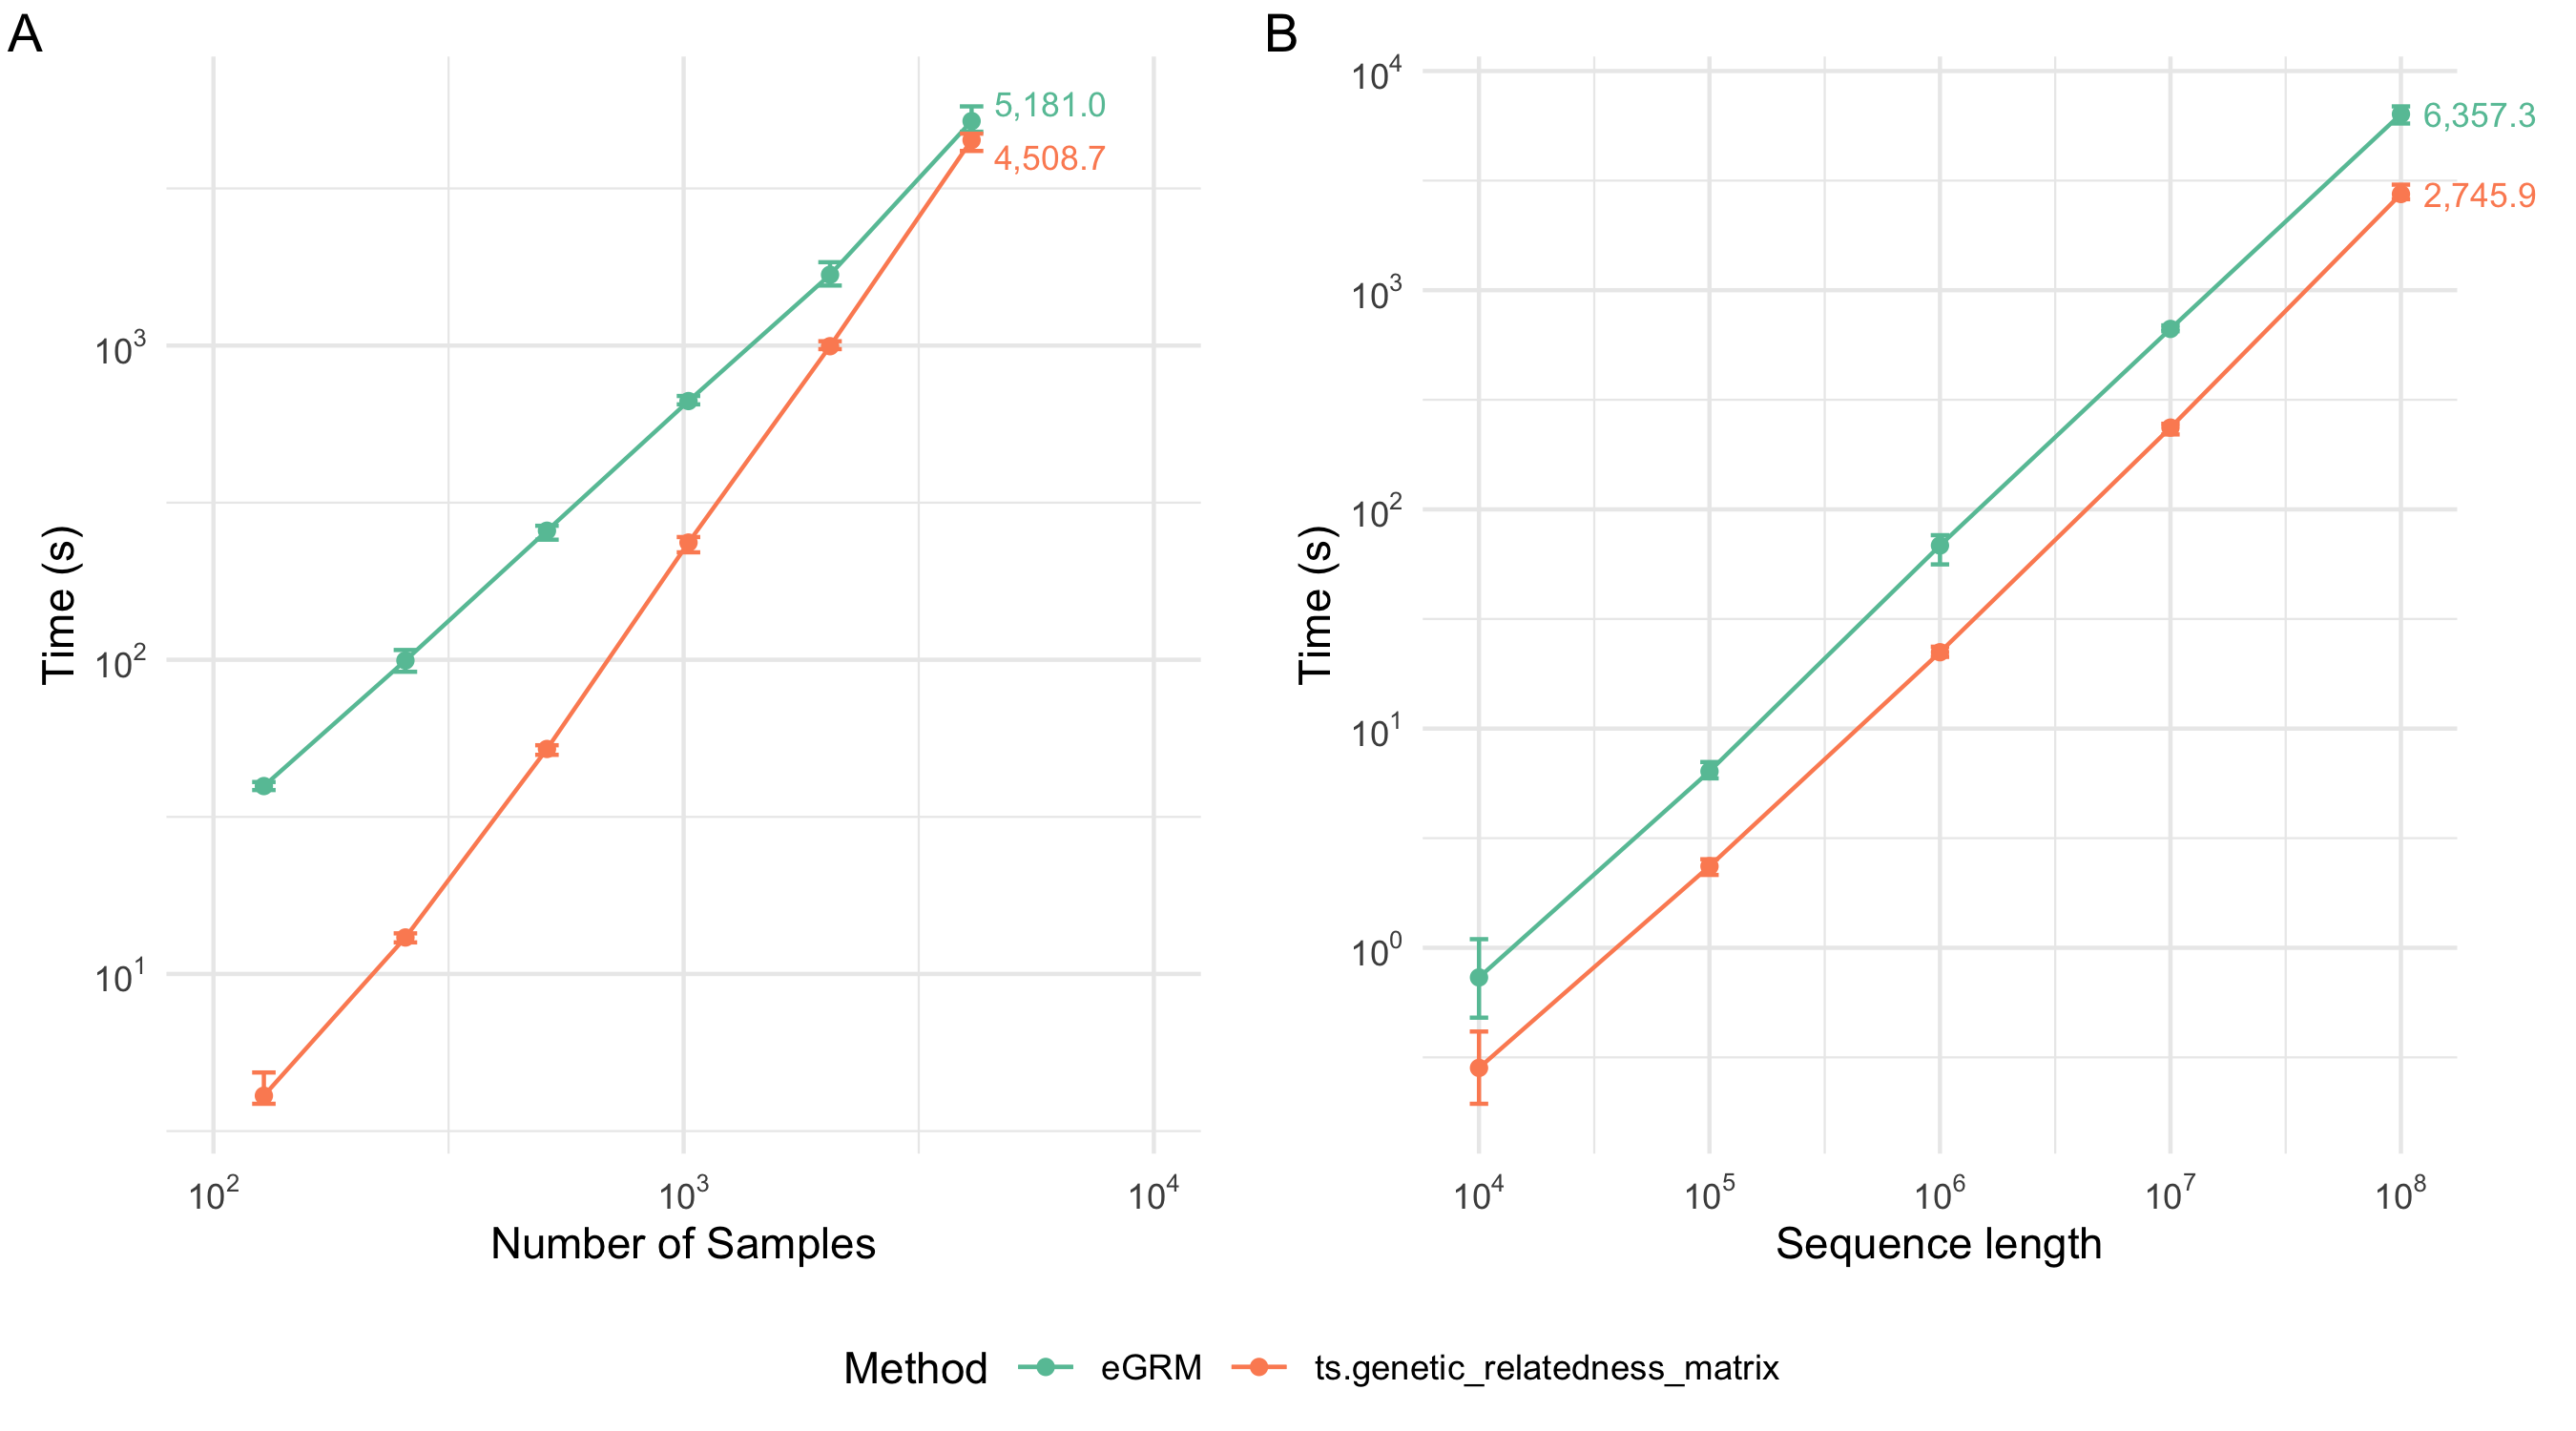
\includegraphics[width=\textwidth]{Figures/SIFig_benchmarking_plot.png}
    \label{fig:SI_benchmarking}
    \caption{Time efficiency of different implementations of branch GRM computation.
    Each dot corresponds to the average time taken across ten simulations with different random seeds.
    Error bars represent the range in time taken across the ten simulations.
    (A) Branch GRM computation with genome sequence length fixed at $10^{7}$ and varying the number of samples.
    (B) Branch GRM computation with number of sample nodes fixed at $2^{10}$ and varying genome sequence length.}
\end{figure}

\section{Proof of correctness of Algorithm V}\label{sec:proof-algv-correct}

Here we prove that when Algorithm V completes, $v(s)$ is equal to the
$s^{\text{th}}$ entry of $\mathbf{C}\mathbf{w}$, as defined
in~\eqref{eq:similar_ralph2020}.
In fact, after each step in the algorithm (i.e., after each addition or removal of an edge), 
it is true that for \textit{every} node $n$, the sum of everything above that node is equal to the weighted sum of covariances
for that node including everything up to that point in the genome.
In other words, for every $n$,
\begin{align} \label{eqn:matvec_consistent}
    S_T(n):=
    \sum_{r \ge_T n} v(r) + z(r)w(r) 
    = 
    \sum_{h:h \le k} (b_h-b_{h-1}) \sum_{r:n \le_{T_h} r} \ell_{T_h}(r) \sum_{t: t \le_{T_h} r} w_t
\end{align}
where $T$ is the current tree.
This statement reduces to our claim that the algorithm is correct because
the final tree is an ``empty'' tree with no edges,
so at the end of the algorithm, the left-hand side is simply $v(n)+z(n)$.
This is again $v(n)$ because $z(n)$ is zero due to $x(n)=b_K$.
The right-hand side is equal to equation 
(\ref{eq:similar_ralph2020}) when $n$ is a sample node.

Each time we add an edge with child $c$ and parent $p$ to the tree (step V2), 
we add the value of $w(n)$ to $p$ and all nodes above $p$ in the tree;
when removing edges we subtract (step V1).
Since $w(n)$ is initialized so that each sample $s$ carries $w_s$, this ensures that $w(n)= \sum_{s \le n} w_s$ at all times [as in \cite{kelleher2016efficient, ralph2020efficiently}].

We prove that equation  (\ref{eqn:matvec_consistent}) is always true by induction.
At the first (empty) tree, this is certainly true,
as both sides are equal to zero.
We now consider \textbf{Step V3}. 
Tree $T$ and the bookkeeping variables $v$, $w$ and $x$ are left constant.
Advancing the position from $k$ to $k+1$ only changes 
$z(s)=\ell_T(s) (b_k - x(s))$ to 
$z'(s)=\ell_{T'}(s) (b_{k+1} - x(s))$.
Therefore, the appended value to the left-hand side is
\begin{align}
    \sum_{r: n \le_T r}z'(r)w(r) - z(r)w(r) = (b_{k+1}-b_{k})
    \sum_{r: n \le_T r} \ell_T(r) w(r)
\end{align}
which is also equal to the added value to the right-hand side.
Note that this is the only step that changes the value of equation (\ref{eqn:matvec_consistent}).

\textbf{Step V1} and \textbf{V2} leave the value of both sides unchanged.
Without the loss of generality, we prove this for \textbf{V2}.
Suppose that we added edge $(c,p)$ where $c$ and $p$ are the child and the parent nodes of the edge, respectively.
We can divide the nodes of $\nodes$ into four categories as (1) the child node $c$, (2) nodes below $c$,  (3) the parent node $p$ and nodes above $p$, and (4) all other nodes. 
The insertion changes the values of the intermediate arrays to $v'$, $w'$, $z'$, and $x'$ following \textbf{V2}.
We denote the new tree resulting from the insertion as $T'$.

Observe that the difference in the left-hand side after $\mathbf{V2}$ is
\begin{align}
    \begin{aligned}
        &\sum_{r:n \le_{T'} r} v'(r) + z'(r)w'(r) 
        - \sum_{r:n \le_{T} r} v(r) + z(r)w(r)
        \\
        &= \sum_{r: n\le_{T'}r, n \nleq_T r } v'(r) + z'(r)w'(r) \\
        &+ \sum_{r: n \le_{T'} r, n\le_T r} v'(r)+z'(r)w'(r)-v(r)-z(r)w(r) \\
        &- \sum_{r: n \nleq_{T'} r, n\le_T r} v(r) + z(r)w(r) \\
        &=  \sum_{r: n\le_{T'}r, n \nleq_T r } v'(r) + z'(r)w'(r)\\
        &+ \sum_{r: n\le_T r} v'(r)+z'(r)w'(r)-v(r)-z(r)w(r)
    \end{aligned}
    \label{preserve_split}
\end{align}
for node $n$.
The last line follows from $\{r: n \le_T r \} \subset \{r: n\le_{T'} r\}$ because $T'$ has more edges than $T$.
Nodes in each category have distinct values for the former and the latter sum of this equation.

The set $\{r: n \le_{T'} r, n \nleq_T r\}$ of the first summation is
\begin{align}
    \begin{cases}
         \{r: p \le_{T'} r\} & \quad \text{$n$ in category (1) or (2)} \\
        \emptyset & \quad \text{$n$ in category (3) or (4)}
    \end{cases}
\end{align}
This is because $p$ and the nodes above $p$ are the nodes that were previously not ancestors in $T$, but became ancestors of $c$ and those below $c$ after the addition of the new edge.
The set is empty for the nodes in the third and the fourth category because their ancestor nodes are unchanged after edge insertion.
Therefore, the first summation is
\begin{align}
    \begin{cases}
        \sum_{r: p \le_{T'} r} v'(r) + z'(r)w'(r) & \quad \text{$n$ in category (1) or (2)} \\
        0 & \quad \text{$n$ in category (3) or (4)}
    \end{cases}
\end{align}

The summand of the second summation $v'(r) + z'(r) - v(r) - z(r)$ is
\begin{align}
    \begin{cases}
    v'(c) - v(c) & \quad \text{$r$ in category (1)} \\
    0 & \quad  \text{$r$ in category (2), (3), or (4)}
    \end{cases} 
\end{align}
For $r=c$ ($r$ is in the first category), it follows from $z(c)=0$ due to $\ell_T(c)=0$ and $z'(c)=0$ due to $x'(c)=b_k$.
All the bookkeeping values of the second and the fourth category is unchanged by \textbf{V2}, so the summand is trivially zero.
When $r=p$ ($r$ belongs to the third category), $v'(r) = v(r) + z(r)w(r)$  and $z'(r)=0$ by the operations $v(r) \pluseq z(r)w(r)$ and $x(r)=b_k$ by \textbf{V2}.
Hence, the second summation is
\begin{align}
    \begin{cases}
        v'(c) - v(c) & \quad \text{$n$ in category (1) or (2)} \\
        0 & \quad \text{$n$ in category (3) or (4)}
    \end{cases}
\end{align}
because the set $\{r: n \le_T r\}$ contains $c$ if and only if $n$ belongs to either the third or the fourth category.
An expression for $v'(c)-v(c)$ comes from the operation $v(c) \minuseq v(r)$ following $v(r) \pluseq z(r)w(r)$ of \textbf{V2}
\begin{align}
    v'(c) - v(c) = - \sum_{r: p \le_{T} r} v(r) + z(r)w(r)
\end{align}

Combining the aforementioned results, we see that equation (\ref{preserve_split}) is 
\begin{align}
    \begin{cases}
        \sum_{r: p \le_{T'} r} v'(r) + z'(r)w'(r) - \sum_{r: p \le_{T} r} v(r) + z(r)w(r) & \text{$n$ $\in$ (1) or (2)} \\
        0 & \text{$n$ $\in$ (3) or (4)}
    \end{cases} 
\end{align}
Both cases reduces to zero because the set of nodes ancestral to $p$ are the same in $T$ and $T'$ ($\{r: p \le_T r\}=\{r: p \le_{T'} r\}$), 
 and $v'(r) = v(r) + z(r)w(r)$ for these nodes due to \textbf{V2} and $z'(r)=0$. 

The right-hand side remains the same because the operation changes nothing in its expression:
it's the working sum until the previous local tree that it does not contain any of 
the components of the current tree that is being modified.
This completes the proof.

% --- Mixed ploidy -------------------------------------------------------

% \subsection{General ploidy}
% \peter{This section to be removed.}

% We now consider the covariance between $p$-ploid individuals,
% possibly different levels of ploidy.
% %
% Returning to the notation for trait in methods, suppose individual $i$ has
% ploidy $p_i$, then their trait genetic value is given by:
% %
% $$ 
% Z(i) = \sum_l \sum_{g=1}^{p_i} Z_{l,G_{i,l,g}}.
% $$
% %
% Let $n_g = \sum_{i=1}^{n_i} p_i$ be the total number of genome copies
% in the sample set of $n_i$ individuals.
% %
% The mean haploid value of the genome copies in individuals $1, \ldots, n_i$
% with genetic values $Z(1), \ldots, Z(n_i)$ is $\bar{Z}_g = (Z(1) + \cdots + Z(n_i))/n_g$.
% %
% If we center the value of each genome copy, then the centered trait value is given by:
% %
% \begin{align}
%   \tilde{Z}(i) &= \sum_{l} \sum_{g=1}^{p_i} \left( Z_{l,G_{i,l,g}} - \bar{Z}_g \right) \\
%                &= \sum_{l} \left( \sum_{g=1}^{p_i} Z_{l,G_{i,l,g}} - p_i\bar{Z}_g \right)
% \end{align}
% %
% Note that when $p_i = p$ for all $i$, then $n_g = n_i \times p$ and
% the above $\tilde{Z}(i)$ is equivalent to $Z(i) - \bar{Z}$.
% %
% This yields a general, including mixed, ploidy version of \eqref{eqn:trait_cov}:
% %
% \begin{align} \label{eqn:trait_cov_mixed}
%     \begin{split}
%         &\Cov\left[ \tilde{Z}(i), \tilde{Z}(j) \right]\\
%         &\qquad = \sum_l \Cov\left[ \left( \sum_{g=1}^{p_i} Z_{l,G_{i,l,g}} - p_i\bar{Z}_g \right)
%                                     \left( \sum_{g=1}^{p_j} Z_{l,G_{j,l,g}} - p_j\bar{Z}_g \right) \right]\\
%         &\qquad = \sigma^2 / 2 \sum_l \sum_a
%                                \left(n(i,l,a) - p_i\bar{n}(l,a)\right)
%                                \left(n(j,l,a) - p_j\bar{n}(l,a)\right).
%     \end{split}
% \end{align}
% %
% This general ploidy formulation opens the opportunity to compute relatedness
% between individuals of any ploidy as well as between sets of individuals
% grouped in some way, say, by population.
% %
% These sets will often vary in size, hence the need for the general ploidy formulation.

% --- Computing with tree statistics -------------------------------------

% \subsection{Computing with tree statistics}
% \label{sec:treestats}

% In summary,
% let $n_g = \sum_{i=1}^{n_i} p_i$ and
% let $\bar{x} = \frac{1}{n_g}\sum_{g=1}^{n_g} x_g$.
% %
% Let
% %
% \begin{align}
%     f_{i,j}(x_1, \ldots, x_{n_i})
%     &= \frac{1}{2} \left(x_i - p_i \bar{x} \right)
%                    \left(x_j - p_j \bar{x} \right)
% \end{align}
% %
% and for each sample node $g$ and individual $i$ let
% $w_{g,i} = 1$ if $g$ is a genome copy of individual $i$, and
% $w_{g,i} = 0$ otherwise.
% %
% Let $T$ be the unpolarised, not span normalised,
% site statistic with the summary function $f_{i,j}$ and a matrix of weights $\mathbf{W}$.
% %
% Then, $T$ is exactly equation \eqref{eqn:trait_cov_mixed} and
% the following equivalences hold:
% %
% \begin{itemize}
%     \item 
%         $T$ is equal to $\Cov\left[Z(i) - \bar{Z}, Z(j) - \bar{Z}\right]$,
%         as in equation \eqref{eqn:trait_cov}.
        
%     \item 
%         If all sites are bi-allelic,
%         and $n_l$ is the number of loci,
%         then $T/n_l = C_{i,j}$,
%         as in equation \eqref{eqn:grm}.
        
%     \item
%         $T$ has the following interpretation:
%         let $m(i ,j)$ denote the total number of pairwise allele matches
%         between the genomes of individual $i$ and of individual $j$,
%         and let $U$ and $V$ be independently chosen individuals from the set of individuals.
%         Then $T$ is the number of pairwise allele matches between $i$ and $j$
%         relative to the rest of the samples:
%         $T = \E[m(i,j) - m(i,U) - m(j,V) + m(U,V)]$,
%         as in equation \eqref{eqn:relative_allele_matches}.
        
% \end{itemize}

% To obtain covariances of the non-centered values
% (i.e., for $Z(i)$ not $Z(i) - \bar Z$),
% one uses
% \begin{align*}
%     f_{i,j}(x_1, \ldots, x_{n_i})
%     = x_i x_j ,
% \end{align*}
% with a \emph{polarised} statistic.

% --- Weighted sums ------------------------------------------------------

% TODO: GG continue parsing/polishing here (see notation.text!)
% N_p --> n_g
% N --> n_i
% I --> i
% J --> i
% i --> ???
% j --> ???

% \subsection{Weighted sums}

% \todo[inline]{TODO: $Z(\mathbf{W})_i$ notation is confusing}

% Let $\mathbf{W}$ be a $n_g \times n_i$ matrix of weights,
% where $n_g$ is the number of genome copies and $n_i$ is number of individuals,
% and let $Z(\mathbf{W})_k = \sum_i \mathbf{W}_{k,i} Z(i)$.
% %
% \todo[inline]{TODO: this $_k$ is confusing because the sum is supposed to go over
% individuals (denoted with $i$) to get $k-$th $Z(\mathbf{W})_k$,
% but unclear what is this quantity!
% Below we have $Z(\mathbf{W})_I$ indicating that $_k$ is indexing individuals,
% but above definition suggests it's sum over individual's values for $k-$th genome?}
% %
% Let $\bar{Z}$ be defined appropriately. (???)
% %
% Let $f_{i,j}$ be as above, and let the weights be given by $\mathbf{W}$.
% %
% Then
% $$
%     T = \Cov\left[Z(\mathbf{W})_I - \bar{Z}, Z(\mathbf{W})_J - \bar{Z}\right] .
% $$
% \todo{TODO: Change $I$ and $J$ to $i$ and $j$ once above confusion is cleared.}
% %
% So, for instance, suppose we want to compute
% $\Cov\left[Z(i), \sum_? w_? Z(?)\right]$, for each $i$.
% %
% Then we would use a matrix of weights $\mathbf{W}$ as above,
% with an extra column for $w$,
% and the summary function
% $(f_{1,n_i+1}, f_{2,n_i+1}, f_{3,n_i+1}, \ldots, f_{n_i, n_i+1})$.
% %
% And figure out what happens with $\bar{Z}$. (???)

% --- Matrix-vector multiplications --------------------------------------

% \subsection{Matrix-vector multiplications}

% In terms of a GP kernel matrix $\mathbf{K}$ on \textit{individuals}
% (rather than haplotypes), we have:
% %
% $$
%     \mathbf{K}_{i,j} = \Cov\left[Z(i) - \bar{Z}, Z(j) - \bar{Z}\right].
% $$
% %
% Or, writing $\tilde{\mathbf{Z}} = (Z(1) - \bar{Z}, \dots, Z(n_i) - \bar{Z})$,
% then $\mathbf{K} = \Var\left[\tilde{\mathbf{Z}}\right] \equiv \Cov\left[\tilde{\mathbf{Z}}, \tilde{\mathbf{Z}}\right]$.

% Suppose we want to evaluate $\mathbf{Kb}$ for a vector $\mathbf{b}$.
% %
% We have:
% %
% $$ \mathbf{Kb} = \Cov\left[\tilde{\mathbf{Z}}, \mathbf{b}^T\tilde{\mathbf{Z}}\right] $$
% %
% So the $i^{th}$ component of $\mathbf{Kb}$ is:
% %
% \begin{align}
%     (\mathbf{Kb})_i &= \Cov\left[ Z(i) - \bar{Z}, ~\sum_{j=1}^{n_i} b_j \left(Z(j) - \bar{Z} \right) \right] \\
%                     &= \Cov\left[ Z(i) - \bar{Z}, ~\sum_{j=1}^{n_i} b_j Z(j) - \sum_{j=1}^{n_i} b_j \bar{Z} \right]
% \end{align}
% %
% Factoring out $\sum{j=1}^{n_i} b_j = B$,
% $$
%     (\mathbf{Kb})_i = B \times \Cov\left[ Z(i) - \bar{Z}, ~\sum_{j=1}^{n_i} (b_j/B) Z(j) - \bar{Z} \right],
% $$
% so $\bar{Z}$ doesn't need changing!(?)

% We also have
% $$
%     (\mathbf{Kb})_i = \sum_{j=1}^{n_i} b_j \Cov\left[ Z(i) - \bar{Z}, ~Z(j) - \bar{Z} \right] 
% $$

% Using equation \eqref{eqn:trait_cov_mixed}:
% %
% % TODO: polish
% \begin{align}
%     (\mathbf{Kb})_i
%         &= \sigma^2 / 2 \sum_{j=1}^N b_j \sum_k \sum_a
%             \left(n_k(I,a) - p_I\bar{n}(k,a)\right) \left( n_k(j, a) - p_j\bar{n}(k,a)\right) \\
%         &= \sigma^2 / 2 \sum_k \sum_a
%             \left(n_k(I,a) - p_I\bar{n}(k,a)\right) \sum_{j=1}^N b_j  \left( n_k(j, a) - p_j\bar{n}(k,a)\right) \\
%         &= \sigma^2 / 2 \sum_k \sum_a
%             \left(n_k(I,a) - p_I\bar{n}(k,a)\right) \left(\sum_{j=1}^N b_j n_k(j, a) - \bar{n}(k,a)\sum_{j=1}^N b_jp_j \right)
% \end{align}

% So, given the weight matrix above, the summary function we want is 
% %
% $$\begin{aligned}
%  f_{i,j}(x_1, \ldots, x_{n_i})
%  &= \frac{1}{2} \left(x_i - \bar{x}\sum_? W_{?,i} \right)
%                 \left(x_j - \bar{x}\sum_? W_{?,j} \right).
% \end{aligned}$$
% %
% This is equivalent to the previous summary function, since $p_i = \sum_? \mathbf{W}_{?,i}$.

% --- Kinship matrices ----------------------------------------------------

% \subsection{Kinship matrices}

% \todo[inline]{Most of this is now in methods.tex! Should we remove this sub-section?}

% One definition of the kinship matrix between individuals $i$ and $j$ is
% that $K_{i,j}$ is equal to
% ``the probability of a match between alleles drawn at random from each of them'',
% averaged over sites and with the alleles drawn with replacement if $i=j$
% (Speed \& Balding, definition of $K_{as}$).
% %
% Note that the probability of a match between two randomly chosen alleles
% is equal to the number of pairwise matches divided by $p^2$,
% where $p$ is the ploidy.
% %
% To get $K_{as}(i,j)$,
% we would take the summary function $x_i x_j$ and divide by $p^2 n_?$.
% %
% Another definition of Speed \& Balding is $K_{c0}$,
% and is equal to equation \eqref{eqn:grm}.

% --- Polarisation -------------------------------------------------------

% \subsection{Polarisation}

% Let $S'$ denote the \emph{polarised} site statistic with
% summary function $f_{i,j}$ and weights $w$.
% %
% This is simply equation \eqref{eqn:compute_C}
% but where the sum is over all \emph{non-ancestral} alleles,
% and so is equal to:
% %
% \begin{itemize}
%     \item
%         The number of pairwise matches of \emph{non-ancestral} alleles between $i$ and $j$
%         relative to random individuals, as above.
%     \item
%         $\Cov[Z(i) - \bar{Z}, Z(j) - \bar{Z}]$
%         instead the ancestral allele has zero effect and
%         derived alleles have variance $\sigma^2 / 2$.
% \end{itemize} 

% Note in particular that if all sites are bi-allelic,
% then the two components of \eqref{eqn:trait_cov} obtained by each of the two alleles are equal
% (since $(a-c)(b-d) = ((n-a)-(n-c))((n-b)-(n-d))$),
% and so the polarised statistic is just equal to one-half of the unpolarised statistic.


\end{document}
